%% ---------------------------------------------------------------------------
%% Economic Forecasting with an Agent-Based Model of the United States
%% MarketsReplica research pipeline, 2026-08-10.
%%
%% Build:  latexmk -pdf -interaction=nonstopmode US_ABM_Forecasting_Paper.tex
%% Figures: python3 ../figures_src/make_figures.py
%% ---------------------------------------------------------------------------
\documentclass[11pt,a4paper]{article}

\usepackage[margin=2.6cm]{geometry}
\usepackage[T1]{fontenc}
\usepackage[utf8]{inputenc}
\usepackage{lmodern}
\usepackage{microtype}
\usepackage{amsmath,amssymb}
\usepackage{booktabs}
\usepackage{array}
\usepackage{graphicx}
\usepackage{xcolor}
\usepackage{tikz}
\usetikzlibrary{arrows.meta,positioning,shapes.geometric,calc,fit,backgrounds}
\usepackage[font=small,labelfont=bf,skip=6pt]{caption}
\usepackage{enumitem}
\usepackage{placeins}
\usepackage{natbib}
\bibliographystyle{plainnat}
\usepackage[hidelinks,breaklinks]{hyperref}

\definecolor{accent}{HTML}{1A4F8A}
\definecolor{accentpale}{HTML}{9DBEDD}
\definecolor{greyrule}{HTML}{8C8C8C}
\definecolor{greypale}{HTML}{E8E8E8}

% compact monospace with automatic underscore handling; \pathc additionally
% permits line breaks inside long artifact paths.
\newcommand{\code}[1]{\texttt{\detokenize{#1}}}
\newcommand{\pathc}[1]{{\urlstyle{tt}\nolinkurl{#1}}}

\emergencystretch=1.6em
\setlength{\tabcolsep}{5pt}
\renewcommand{\arraystretch}{1.08}
\newcolumntype{R}{>{\raggedleft\arraybackslash}X}

\newcommand{\pp}{\,pp}
\title{\bfseries Economic Forecasting with an Agent-Based Model\\ of the United States:\\
\large Calibration, Diagnosis, and Out-of-Sample Performance}

\author{MarketsReplica research pipeline}
\date{10 August 2026}

\begin{document}
\maketitle

\begin{abstract}
\noindent
We port the agent-based macroeconomic model of \citet{poledna2023} to the United States and
subject it to that paper's own out-of-sample protocol: 61 quarterly forecast origins from
2010Q2 to 2025Q2, horizons of 1, 2, 4, 8 and 12 quarters, 500 free-running stochastic paths per
origin, and ten statistical benchmarks scored on identical cells. The first pass produced a
defect rather than a result: real GDP growth was under-forecast by 1.3 to 2.9 percentage points
at every horizon. We trace it by matched-seed experiment to the calibration artifact's opening
commodity balance, which does not clear sector by sector --- modelled uses differ from supply by
$-70.6\%$ to $+47.6\%$ across 68 commodities --- colliding with a firm capacity envelope frozen at
$K_i\kappa_i = Y_i/0.85$ because investment is replacement-only. Over-demanded sectors sit
permanently against their ceiling, under-demanded ones permanently idle, and the one-sided
production constraint prevents the idle capacity from compensating. This accounts for 76\,\% of
the bias; a growth expectation estimated by ordinary least squares AR(1) on the \emph{log level}
of an I(1)-with-drift series, which delivers only 32--63\,\% of the in-sample trend, accounts for
the remainder. We repair both on accounting grounds alone --- biproportional (RAS) reconciliation
of the use side that retains measured BEA imports, and a random-walk-with-drift expectation ---
with neither repair \emph{selected} using forecast errors, and re-score on identical cells
with identical seeds. The exercise remains explicitly mixed-vintage: 2024 structure and
current-vintage data are used at historical origins. The repaired model attains the best weighted RMSE ratio of all fourteen
scored columns on \{real GDP growth, GDP-deflator inflation\} in all three sample tracks (0.830,
0.829 and 0.796 against a VAR(1) anchor); real-GDP bias falls below $0.21$ percentage points at
every horizon and empirical 90\,\% interval coverage moves from 0.654 to 0.929. The GDP deflator
is unchanged, and bit-identical at $h=1$, which is the signature the diagnosis predicted. Two
measured defects bound every number: capital never accumulates, so growth drains a fixed 17.6\,\%
capacity headroom and the result is validated only to $h\le 12$; and unemployment collapses to
about 1\,\%, is excluded from every weighted score, and became worse. This is a revised-data,
mixed-vintage diagnostic, not a real-time forecasting claim.
\end{abstract}

\medskip
\noindent\textbf{Keywords:} agent-based macroeconomics; out-of-sample forecast evaluation;
input--output reconciliation; supply--use balance; model diagnosis.

\vspace{1em}
\hrule
\vspace{0.6em}
\noindent\small
\textbf{Reader's note.} This paper is written for a technically trained reader who is not an
economist by training. Economic machinery is defined at first use, and the accounting identities
that carry the argument are written out rather than assumed. Every number is traceable to a
committed artifact; Appendix~\ref{app:repro} gives the paths, hashes and commands.
\normalsize
\vspace{0.6em}
\hrule

\clearpage

% ===========================================================================
\section{Introduction}
\label{sec:intro}

\subsection{The Poledna programme}

Macroeconomic forecasting is dominated by two model classes. \emph{Time-series} models --- vector
autoregressions (VARs) and their Bayesian variants --- treat the economy as a low-dimensional
stochastic process and extrapolate its estimated dynamics; they are accurate at short horizons
and structurally mute. \emph{Dynamic stochastic general equilibrium} (DSGE) models
\citep{smetswouters2007} write down a small number of optimising representative agents, impose
market clearing at every date, and estimate the resulting cross-equation restrictions; they are
structurally interpretable and, at forecast horizons, rarely better than a well-specified VAR.

\emph{Agent-based models} (ABMs) take a third route \citep{farmerfoley2009}. They simulate a
population of heterogeneous entities --- firms, households, a bank, a government --- each following
explicit behavioural rules, and let aggregates emerge from decentralised interaction. Markets do
not clear by assumption; they clear, or fail to clear, through search and matching, with rationing
as an observable outcome. For two decades this class was excluded from the forecasting
conversation on the grounds that it was unfalsifiable in the only way that matters: nobody had run
one against the standard benchmarks on a rolling out-of-sample grid.

\citet{poledna2023} closed that gap. They calibrated a large ABM of Austria one-to-one against the
national accounts, ran free-running forecasts from quarterly origins over 2010Q2--2016Q4 at
horizons $h \in \{1,2,4,8,12\}$ with 500 stochastic paths each, and scored the ensemble mean
against AR, VAR and Bayesian DSGE benchmarks. The ABM was competitive, and better than the DSGE at
most horizons. That result is the reference point of the present work, and its protocol is the one
reproduced here.

\subsection{What this paper does}

This paper reports a port of that programme to the United States, and it reports what the port
found. The arc is: \emph{built} $\rightarrow$ \emph{scored} $\rightarrow$ \emph{found defective}
$\rightarrow$ \emph{diagnosed} $\rightarrow$ \emph{repaired on accounting grounds} $\rightarrow$
\emph{re-scored on identical cells}. That arc, and not the rank it terminates in, is the
contribution.

\begin{enumerate}[leftmargin=1.4em,itemsep=2pt]
\item \textbf{Port and first-pass validation} (\S\ref{sec:calib}--\S\ref{sec:design}). The
      BeforeIT implementation \citep{beforeit2025} of the Poledna model is calibrated against the
      U.S.\ Bureau of Economic Analysis (BEA) supply--use system and run over 61 quarterly
      origins, 2010Q2--2025Q2, at $h\in\{1,2,4,8,12\}$ with 500 paths per origin and zero path
      failures, against ten statistical benchmarks on matched cells.
\item \textbf{Defect discovery} (\S\ref{sec:v1}). The first-pass model (\code{beforeit_abm_us_v1})
      is competitive on the full sample and eleventh of fourteen once the pandemic cells are
      removed, and it under-forecasts real GDP growth by $1.3$ to $2.9$ percentage points at every
      horizon.
\item \textbf{Diagnosis} (\S\ref{sec:diagnosis}). Matched-seed experiments attribute 76\,\% of the
      bias to a non-clearing opening commodity balance colliding with a frozen capacity envelope,
      and 24\,\% to a misspecified growth-expectation estimator, with an explicit falsification
      table for the competing hypotheses.
\item \textbf{Structural repair} (\S\ref{sec:repair}). Both defects are corrected in the
      calibration artifact using past-only information and no reference to any forecast error: a
      biproportional (RAS) reconciliation of the use side that retains the measured import levels,
      and a random-walk-with-drift growth expectation.
\item \textbf{Re-validation} (\S\ref{sec:v2}). The repaired model (\code{beforeit_abm_us_v2}) is
      scored jointly with the unrepaired one, on identical common cells with identical random
      seeds, in a single run.
\end{enumerate}

\subsection{What the reader should take away, and what they should not}

The repaired model ranks first of fourteen on the headline target pair in all three sample tracks.
That is a real result on a matched grid, and it is also a \emph{revised-data, mixed-vintage
diagnostic}: the data are current-vintage throughout, and the input--output structure is frozen at
2024 and carried backwards to every historical origin. No real-time information set was
reconstructed, no DSGE benchmark is in the field, and no formal forecast-comparison inference was
performed, so adjacent ranks are not statistically distinguishable. Two open defects --- capital
that never accumulates and a labour block that overheats after the repair --- bound the validity of
every number reported here. These limits are stated in \S\ref{sec:limits} and are not incidental
to the result; they are part of it.

% ===========================================================================
\section{The model}
\label{sec:model}

This section is a compact overview sufficient to read the results. The full equation system is in
\citet{poledna2023} and its implementation in \citet{beforeit2025}; nothing in the behavioural
block was modified for this work except the one flag-gated expectation change documented in
\S\ref{sec:repair}.

\subsection{Agents and the flow of a quarter}

The economy contains six classes of agent.

\begin{description}[leftmargin=1.6em,style=nextline,itemsep=3pt]
\item[Firms.] $\sum_s I_s$ firms distributed over $S$ industries. Each firm $i$ in industry $s$
  produces a single commodity with a \emph{Leontief} technology \citep{leontief1936}: output
  requires labour, intermediate inputs and capital services in fixed proportions, with no
  substitution between them. Concretely, output is capped by the binding factor,
  \begin{equation}
    Y_i = \min\!\Big( \underbrace{\alpha_s N_i}_{\text{labour}},\;
                      \underbrace{\beta_s M_i}_{\text{materials}},\;
                      \underbrace{\kappa_s K_i}_{\text{capital}} \Big),
    \label{eq:leontief}
  \end{equation}
  where $N_i$ is employment, $M_i$ the intermediate-input bundle, $K_i$ the capital stock, and
  $(\alpha_s,\beta_s,\kappa_s)$ are industry productivities read off the input--output table. The
  third term is the \emph{capacity envelope}; it is the object at the centre of
  \S\ref{sec:diagnosis}.
\item[Households.] Worker households supply labour and consume; inactive households receive
  transfers and consume; firm owners receive dividends. Consumption follows a propensity rule on
  disposable income and liquid wealth, allocated across commodities by a fixed basket $b^{HH}_g$.
\item[A bank.] One consolidated commercial bank intermediates deposits and loans subject to a
  capital-adequacy constraint, and rations credit when the constraint binds.
\item[A central bank.] Sets the policy rate by a Taylor rule --- a feedback rule raising the rate
  when inflation or an activity measure exceeds target --- with inertia $\rho$, an intercept
  $r^{*}$, and response coefficients $\xi_\pi$ and $\xi_\gamma$.
\item[A government.] Collects taxes, pays wages, transfers and unemployment benefits, consumes a
  commodity basket $c^{G}_g$, and issues debt.
\item[A rest-of-world block.] Exports absorb a basket $c^{E}_g$; imports supply $c^{I}_g$. In this
  calibration the block is exogenous and is driven by estimated univariate processes.
\end{description}

Within a quarter, firms form expectations, choose target output and desired inputs, post vacancies
and demand credit; the labour, credit and goods markets then clear through decentralised
\emph{search and matching} --- buyers meet a random subset of sellers, transact at posted prices,
and any unmet demand is simply not satisfied. Rationing is therefore a first-class observable of
the model, reported here as \emph{fill rates}. Insolvent firms exit and are replaced.

\subsection{The behavioural core in five equations}

Table~\ref{tab:equations} lists the equations that carry the argument of this paper. The remaining
several dozen --- price and wage setting, credit allocation, the bank's balance sheet, the fiscal
block --- are unchanged from the reference implementation and are not reproduced.

\begin{table}[t]
\centering
\caption{The five model relations that the diagnosis of \S\ref{sec:diagnosis} turns on.
Notation follows \citet{poledna2023}; $\delta_s$ is the depreciation rate, $\omega$ the assumed
normal capacity utilisation, $Q^d_i$ desired sales and $Q^s_i$ target production.}
\label{tab:equations}
\small
\begin{tabular}{@{}p{0.30\textwidth}p{0.63\textwidth}@{}}
\toprule
\textbf{Relation} & \textbf{Form and role} \\
\midrule
Production, Leontief with a capacity cap &
$Y_i=\min(\alpha_s N_i,\;\beta_s M_i,\;\kappa_s K_i)$. The $\min$ is \emph{one-sided}: a firm
below its cap cannot lend spare capacity to a firm above it. \\[2pt]
Target output &
$Q^s_i = Q^d_i\,(1+\gamma_e)$, where $\gamma_e$ is the economy-wide expected growth rate. \\[2pt]
Growth expectation (v1) &
$\gamma_e=\exp(\hat\alpha \log Y_{\text{last}}+\hat\beta)/Y_{\text{last}}-1$ with
$(\hat\alpha,\hat\beta)$ from an OLS AR(1) with constant on the \emph{log level} of the model's own
aggregate output history. \\[2pt]
Desired investment &
$I^d_i=(\delta_i/\kappa_i)\min(Q^s_i,\;K_i\kappa_i)$, and
$K'=K-(\delta/\kappa)Y+I$. When firms obtain their desired investment and produce at target these
give $K'=K$ exactly: investment is \emph{replacement-only}. \\[2pt]
Opening capacity &
$\kappa_s=\tau\,\text{(industry output)}/\text{(fixed assets)}/\omega$ and $K_i=Y_i/(\omega\kappa_i)$,
so $K_i\kappa_i=Y_i/\omega$ identically. With $\omega=0.85$ every firm opens at 85\,\% utilisation
with $1/0.85-1=17.6\,\%$ headroom. \\
\bottomrule
\end{tabular}
\end{table}

Two properties of Table~\ref{tab:equations} interact destructively, and \S\ref{sec:diagnosis} is
about that interaction. First, the capacity envelope $K_i\kappa_i$ is fixed at construction in
proportion to the \emph{opening output composition}. Second, because investment is
replacement-only, it never moves: measured over every experimental variant run for this paper,
$K_{\text{end}}/K_1 = 1.0000$--$1.0009$. The capacity vector is therefore a constant, and the
demand vector it must serve is a different constant, determined by the technology and final-demand
coefficient matrices $(a_{sg}, b^{HH}_g, b^{CF}_g, c^{G}_g, c^{E}_g)$. If the two are inconsistent,
nothing in the model can reconcile them.

The replacement-only investment rule is inherited from the upstream implementation, not introduced
by this fork; the $\min(\cdot)$ in the desired-investment equation was already present in the
upstream commit that this fork descends from.

% ===========================================================================
\section{United States calibration and data}
\label{sec:calib}

\subsection{The calibration artifact}

A \emph{calibration artifact} is a single serialised object holding every parameter and initial
condition the simulator needs: the technology matrix, final-demand baskets, agent counts, tax and
benefit rates, opening stocks, and the quarterly exogenous series. It is built once from public
data and then loaded read-only by the forecasting harness.

The classification comes from the BEA summary-level supply--use system \citep{bea_io}. That source
carries 68 observed commodities and 71 industries; the four retail industry columns
(\code{441}, \code{445}, \code{452}, \code{4A0}) are summed into a single model sector \code{4A0},
giving 68 modelled industries matched one-to-one against the 68 commodities. Table~\ref{tab:calib}
gives the resulting dimensions.

\begin{table}[t]
\centering
\caption{United States calibration at $\text{scale}=10^{-5}$. One modelled firm stands for
$10^{5}$ real ones; the reference Austrian exercise ran at 1:1.}
\label{tab:calib}
\small
\begin{tabular}{@{}lr@{\qquad}lr@{}}
\toprule
Commodities $G$ & 68 & Economically active households $H^{\mathrm{act}}$ & 1\,826 \\
Industries $S$ (from 71 BEA industries) & 68 & Inactive households $H^{\mathrm{inact}}$ & 1\,005 \\
Firms $\sum_s I_s$ & 130 & Total population represented & $\approx 2\,831$ \\
Government entities $J$ & 33 & Foreign consumers $L$ & 65 \\
\midrule
\multicolumn{4}{@{}l}{Runtime: 0.085\,s per 12-quarter path after compilation, single-threaded.}\\
\bottomrule
\end{tabular}
\end{table}

\subsection{United States--specific choices in the artifact}

Four choices depart from the reference specification and matter for what follows.

\begin{description}[leftmargin=1.4em,style=nextline,itemsep=3pt]
\item[Explicit measured trade (\code{use_explicit_trade = true}).] Commodity imports are taken
  from the measured BEA T262 import matrix rather than being solved as the supply--use residual.
  This preserves the measured import level and is closer to the reference paper's stated intent of
  reading trade off the input--output table --- but it leaves the sector-level balance
  unreconciled. This is the single most consequential U.S.-specific choice in the artifact and it
  is the subject of \S\ref{sec:diagnosis}. The repair \emph{retains} it.
\item[Product-tax netting (\code{use_product_tax_netting = true}).] A valuation bridge, discussed
  in \S\ref{sec:austria}.
\item[Discrepancy-derived opening inventories.] In the first-pass artifact,
  \code{use_commodity_balance_inventory = true} derives opening sector inventories $S_s$ from the
  positive part of the negated statistical discrepancy. The pipeline source sets this flag to
  \code{false}; the artifact and the pipeline disagreed, and the artifact won for every origin the
  harness built. The repaired artifact sets it \code{false}, removing both the accuracy defect and
  the reproducibility hazard.
\item[Policy rate on a quarterly basis.] The legacy field named \code{euribor} holds the U.S.\
  policy rate, stored as $r=(\text{annual rate}+1)^{1/4}-1$. Comparison against the
  annualised-percentage-point effective federal funds rate (EFFR) therefore requires
  $100\,((1+r)^4-1)$. At 2024Q4 this gives 4.571\,\% against a panel value of 4.65\,\%.
\end{description}

\subsection{The no-fitting firewall}

That behavioural parameters have \emph{not} been fitted to forecast errors was verified rather than
assumed. The stored baseline carries firewall metadata recording that the parameters are raw,
that no forecast-error-fitted parameters are present
(\code{forecast_error_fitted_parameters = false}) and that no post-processing is embedded, with
four restored parameters and seven removed output corrections. Numerically, at 2024Q4 the four
Taylor-rule parameters take the values in Table~\ref{tab:firewall}; all $\approx70$ parameter keys
agree between the stored baseline and a fresh derivation, neither equals the discarded
forecast-fitted overrides, and the two produce bit-identical 12-quarter paths under the same seed.

\begin{table}[t]
\centering
\caption{Raw-dynamics firewall check at 2024Q4. The right-hand column is the discarded
forecast-error-fitted override layer, retained only for contrast; no result in this paper reads it.}
\label{tab:firewall}
\small
\begin{tabular}{@{}lrrr@{}}
\toprule
Parameter & Stored baseline & Fresh derivation & Discarded fitted override \\
\midrule
$\rho$        & 0.954811254910 & 0.954811254910 & 0.911458333333 \\
$r^{*}$       & $-0.001043926436$ & $-0.001043926436$ & $-0.002333333333$ \\
$\xi_\pi$     & 0.789655283206 & 0.789655283206 & 0.708333333333 \\
$\xi_\gamma$  & 0.532167779487 & 0.532167779487 & 0.258730279487 \\
\bottomrule
\end{tabular}
\end{table}

The firewall applies with equal force to the repair of \S\ref{sec:repair}. Both changes restore an
accounting identity or correct an estimator that is wrong on its own terms, using past-only
information. Re-estimating $\omega$, the Taylor-rule coefficients or the expectation parameters
against realised GDP paths would be behavioural tuning; it is named here explicitly as prohibited,
and it was not done.

\subsection{Absence of behavioural look-ahead}

The exogenous arrays for government consumption, exports and imports extend up to twelve quarters
past each origin in the artifact. This is behaviourally empty: only the element at the origin index
is ever read, once, as a scalar, at construction, after which the series evolve by their own
estimated processes. The claim was tested by mutation. Three runs at 2024Q4 under an identical seed
--- untruncated; truncated to the origin; and untruncated with \emph{every post-origin entry
overwritten by $-10^{99}$} --- produced bit-identical real GDP, nominal GDP and policy-rate paths,
with the poisoned run finite throughout. Truncation is applied anyway as past-only hygiene, and
every estimation window terminates at the origin.

% ===========================================================================
\section{From Austria to the United States: what had to change, and why it was hard}
\label{sec:austria}

The reference exercise is Austrian. Porting it is often described as a data-substitution task. It
is not, and the difference is the origin of the defect diagnosed in \S\ref{sec:diagnosis}.

\subsection{A side-by-side comparison}

\begin{table}[t]
\centering
\caption{Structural differences between the reference Austrian calibration and the United States
calibration used here. The right-hand column is not a list of approximations to be tightened
later; several entries change what the model can be asked to do.}
\label{tab:austria-us}
\footnotesize
\begin{tabular}{@{}p{0.155\textwidth}p{0.38\textwidth}p{0.40\textwidth}@{}}
\toprule
& \textbf{Austria (reference)} & \textbf{United States (this work)} \\
\midrule
Input--output source
& Eurostat 64-category NACE/CPA product-by-product tables at \emph{basic prices}, already
  symmetric and balanced \citep{eurostat_naio}
& BEA 71-industry $\rightarrow$ 68-commodity make--use system, published at
  \emph{purchasers' prices}, requiring a valuation bridge and an industry$\rightarrow$commodity
  projection \citep{bea_io} \\[3pt]
Firm counts
& Business demography: active enterprises per sector
& Census Statistics of U.S.\ Businesses \citep{census_susb} plus USDA farm counts and
  pseudo-producers; a mixed enterprise/establishment ontology \\[3pt]
Agent scale
& Approximately 1:1 with observed entities
& $10^{-5}$: 130 firms, $\approx 2\,831$ modelled people; \textbf{54 of 68 sectors hold exactly one
  firm} \\[3pt]
Foreign block
& Euro-area output and inflation are genuinely \emph{exogenous} to Austria
& The ``euro-area'' block is filled with \emph{U.S.} data, so the Taylor rule reacts to an
  exogenous proxy for the same economy the model is simulating; there is no independent foreign
  demand state and no policy feedback loop \\[3pt]
Labour and financial accounts
& Harmonised Eurostat sector accounts, one vintage, one classification
& CPS, CES and QCEW surveys stitched to the Financial Accounts (Z.1) across
  different statistical universes \citep{bls_data,frb_z1} \\[3pt]
Unemployment insurance
& A single national replacement rate
& State-level programmes varying by wage, duration and emergency extension; the Austrian constant
  $\theta^{UB}=0.55(1-\tau^{INC})(1-\tau^{SIW})$ survives unchanged in the code \\[3pt]
Trade closure
& Imports read off the balanced table; the balance clears by construction
& Imports measured from BEA T262 while the supply--use residual is \emph{not} re-absorbed, so the
  residual survives as a signed sector-level gap \\[3pt]
Structural vintage
& Structure recalculated at or near each forecast origin
& \textbf{One} 2024 structural row carried backwards to all 61 origins \\
\bottomrule
\end{tabular}
\end{table}

\subsection{Why each difference is hard, not merely different}

\paragraph{Valuation bases.} A supply--use system can be stated at \emph{basic prices} (what the
producer receives) or at \emph{purchasers' prices} (what the buyer pays, including trade and
transport margins and net product taxes). The model's coefficients are defined on the basic-price
convention; the BEA tables are published at purchasers' prices. Bridging requires netting product
taxes and reallocating margins, and every bridge leaves a residual somewhere. Eurostat hands the
Austrian calibration a table that is already on the required basis; the U.S.\ calibration has to
construct one.

\paragraph{The industry/commodity axis.} Eurostat publishes symmetric product-by-product tables:
rows and columns index the same 64 objects. BEA publishes a \emph{make} table (which industry
produces which commodity) and a \emph{use} table (which industry consumes which commodity) over
non-identical axes --- 71 industries against 68 commodities. Projecting one onto the other is a
modelling choice, not a lookup, and it is where an industry-output control and a commodity-row
control can silently end up compared to each other.

\paragraph{One structural year for fifteen years of origins.} The U.S.\ artifact contains 37 annual
arrays of length one, all frozen at 2024: the entire input--output block, firm counts, employees,
population, census unemployed and inactive, fixed assets, dwellings, capital consumption, every tax
and benefit aggregate, and sectoral wages. Out of the box only nine origins are constructible.
Unlocking the historical grid required a single-array rewrite --- shallow-copying the calibration
dictionary and setting the year index to the origin's year, which makes the calibration index
resolve to 1, the only valid index for a length-one array. All quarterly series already run from
1996Q4, so opening \emph{levels} do scale with the era (model opening real GDP is
$5.483\times10^{6}$ at 2019Q4, $3.745\times10^{6}$ at 2010Q2 and $3.231\times10^{6}$ at 2005Q2).
The consequence is a clean and declarable split, which the results tables respect:

\begin{itemize}[leftmargin=1.4em,itemsep=1pt]
\item \textbf{Flow targets} --- real GDP growth, deflator inflation, nominal GDP growth, the policy
  rate --- are initialised from quarterly series with full history. The 2024 structure enters as a
  fixed technology and demand-composition matrix, not as a level. Scoring them is defensible as a
  diagnostic.
\item \textbf{Stock-initialised targets} --- unemployment above all --- open at the 2024 level at
  \emph{every} origin. Scoring them is not defensible, and \S\ref{sec:unemployment} documents the
  failure quantitatively.
\end{itemize}

\paragraph{And therefore the trade-closure problem.} Put the three previous paragraphs together.
A published supply--use system balances by construction, but only in the valuation basis and on the
axes in which it was published. Once the U.S.\ system has been bridged across valuation bases and
projected from industries onto commodities, the balance is no longer guaranteed --- and the
artifact's decision to take imports from the measured T262 matrix, rather than solving them as the
residual, removes the one remaining degree of freedom that could have absorbed the difference. The
residual therefore survives into the simulator as a signed, sector-level gap. That is the defect,
and \S\ref{sec:diagnosis} measures it.

% ===========================================================================
\section{Scientific assumptions register}
\label{sec:assumptions}

Every assumption on which a reported number depends is listed here with its justification and its
status. \textbf{[S]} marks a structural choice --- one that restores an accounting identity or
corrects an estimator that is wrong on its own terms, using past-only information. \textbf{[T]}
would mark behavioural tuning against forecast performance; no entry carries it, and none was done.

\begin{enumerate}[label=\textbf{A\arabic*.},leftmargin=2.6em,itemsep=4pt]

\item \textbf{Revised-data protocol; current-vintage truth, symmetric across models.} The scoring
panel is a current-vintage snapshot of 101 quarters, 2000Q3--2025Q3, used for both estimation and
truth by all fourteen models. Real GDP growth for 2010Q2 is the value as revised through 2026, not
the value available in 2010. \emph{Status:} a known limitation, symmetric across every model, and
the same design the reference paper adopts for the bulk of its evaluation. \emph{Flags:}
\code{real_time = false}, \code{origin_admissible = false}, \code{promotion_eligible = false}.

\item \textbf{2024 structure at every historical origin.} The 37 frozen annual arrays constitute
future information at every origin before 2024. \emph{Status:} asymmetric and ours alone --- the
sharpest departure from the reference paper. Bounded for flow targets; fatal for stock-initialised
targets, which is why unemployment is excluded from every weighted score.

\item \textbf{Agent scale $10^{-5}$.} 130 firms. \emph{Justification:} an agent-count sweep from
130 to 2\,708 firms leaves the truncated-output share at 14\,\% and mean growth near zero, so the
central result is scale-invariant. \emph{Status:} adequate for the mean, \emph{inadequate for
dispersion}: 54 of 68 sectors hold exactly one firm at this scale.

\item \textbf{Normal capacity utilisation $\omega=0.85$ [S, inherited].} Hard-coded upstream. It
fixes opening headroom at $1/0.85 - 1 = 17.6\,\%$ for every firm by construction.
\emph{Status:} an inherited magic number. Sourcing it from the Federal Reserve G.17 capacity
utilisation series \citep{frb_g17} would be a structural improvement; sweeping it to improve RMSE
would be tuning and is prohibited.

\item \textbf{Opening inventories $S_i(0)=0$ after reconciliation [S].} The first-pass artifact set
$S_s = \tau \cdot \max(0, -\text{discrepancy})$, so only the 42 negative-gap sectors received an
opening buffer and the 26 positive-gap sectors received exactly zero; the total was 7.4\,\% of
quarterly gross output with 31\,\% of it in a single sector. \emph{Justification:} a signed
accounting residual is not an inventory stock, and the rule was asymmetric. After the balance
clears there is no signed discrepancy to promote, and the reference specification opens with
$S_i(0)=0$.

\item \textbf{Production-account anchoring, $\lambda = 0.983460$ [S].} Biproportional
reconciliation requires that row controls and column controls sum to the same total. In the
artifact they do not: uses exceed supply by 1.0104\,\% in aggregate. That residual decomposes
\emph{exactly} --- to $5.6\times10^{-9}$ --- into two measurement facts of the source data, shown in
Table~\ref{tab:lambda}. One control must therefore move, and the repair anchors on the production
account, scaling the four final-demand aggregates (and the two components that set the investment
budget) by
\[
  \lambda \;=\; \frac{\text{supply} - \text{intermediates}}{C+G+I+X} \;=\; 0.983460 .
\]
\emph{Status:} $\lambda$ is fixed by the accounting identity alone and was not chosen with
reference to any forecast error. The semantics are recorded verbatim in every result manifest. The
alternative closure --- hold every measured budget and let a uniform 1.01\,\% excess-demand wedge
survive --- was built and measured too; it overshoots, because a uniform 1\,\% excess demand is
itself a growth impulse (\S\ref{sec:headroom}).

\item \textbf{Random-walk-with-drift growth expectations [S].} The first-pass expectation is an OLS
AR(1) with constant fitted to the \emph{log level} of an I(1)-with-drift series. For a log-linear
trend $x_t = a + g t$, OLS gives $\hat\beta = \bar x_t - \hat\alpha \bar x_{t-1}$ and hence the
closed form
\begin{equation}
  \gamma_e \;\approx\; g\Big[\,1-(1-\hat\alpha)\tfrac{T}{2}\,\Big].
  \label{eq:gammae}
\end{equation}
The shrinkage is unavoidable: $\hat\alpha$ carries the Kendall small-sample downward bias
\citep{kendall1954}, and the level shocks of 2008--09 and 2020 push it further down. Shorter
windows do not help --- they trade a smaller $T$ against a more biased $\hat\alpha$.
Table~\ref{tab:gammae} shows the estimator delivering 32--63\,\% of the in-sample trend at every
origin, and Eq.~\eqref{eq:gammae} reproducing it to 0.05\pp. \emph{Status:} a specification
correction, estimated on past data only. Gated behind a model property that is \emph{default-off},
so the Austrian and Italian calibrations remain bit-identical.

\item \textbf{Replacement-only investment [inherited, unrepaired].} $K'=K$ exactly when firms
obtain desired investment and produce at target. \emph{Status:} an upstream design property, not a
fork bug, and \emph{not} repaired here. It is the binding limitation on forward use
(\S\ref{sec:headroom}).

\item \textbf{No behavioural fitting.} Verified numerically (\S\ref{sec:calib}); the forecast-error
override layer is never read on the paths that produce these results.

\item \textbf{Unemployment excluded from every weighted score.} Recorded in each manifest with the
reason: the initial unemployed stock is a length-one annual array frozen at 2024, so every
historical origin opens at the 2024 labour market. It is emitted and diagnosed
(\S\ref{sec:unemployment}) but never scored.

\item \textbf{Seeds and Monte-Carlo policy.} Simulation seeds are
\[
  \mathrm{seed}(\text{origin},\text{path}) \;=\;
  \mathrm{hash}\big((\texttt{:abm\_revised\_v1},\,\text{origin},\,\text{path})\big) \bmod 2^{30},
\]
so no two cells share a stream. The repaired model draws the \emph{identical} seed stream as the first pass,
which makes the contrast matched-seed; the expectations patch consumes exactly one Normal variate
on either branch precisely to preserve that alignment. Failed paths are counted and left visible,
never resampled; the count is zero everywhere.
\end{enumerate}

\begin{table}[t]
\centering
\caption{Exact decomposition of the aggregate excess of uses over supply in the first-pass
artifact. Both terms are measurement facts of the source data, not model choices; neither can be
removed without moving a measured control. Units are millions of current U.S.\ dollars.}
\label{tab:lambda}
\small
\begin{tabular}{@{}lr>{\raggedright\arraybackslash}p{0.38\textwidth}@{}}
\toprule
Term & Value (US\$m) & Meaning \\
\midrule
Expenditure GDP $-$ production GDP & 442\,933 & the artifact's own statistical discrepancy,
1.57\,\% of GDP \\
Capital consumption $-$ non-dwelling GFCF & 88\,223 & net non-dwelling fixed investment is negative
in the artifact \\
\midrule
\textbf{Total} & \textbf{531\,156} & $=\mathrm{sum(uses)}-\mathrm{sum(supply)}$, matched to
$5.6\times10^{-9}$ \\
\bottomrule
\end{tabular}
\end{table}

\begin{table}[t]
\centering
\caption{The growth-expectation estimator, measured at six origins. $T'$ is the length of the
model's own output history at the origin; $\hat\alpha$ is the fitted AR(1) coefficient on the log
level. The last column is the fraction of the in-sample trend that the expectation delivers.
Pinning $\hat\alpha=1$ --- a random walk with drift, using the same past-only data --- recovers
$+2.33$, $+2.39$, $+2.36$, $+2.42$, $+2.37$ and $+2.40\,\%$: the trend, at every origin.}
\label{tab:gammae}
\footnotesize
\begin{tabular}{@{}lrrrrr@{}}
\toprule
Origin & $T'$ & $\hat\alpha$ & $\gamma_e$ (\%) & trend (\%) & $\gamma_e/\text{trend}$ \\
\midrule
2012Q4 & 64  & 0.9713 & $+0.745$ & $+2.331$ & 0.32 \\
2014Q4 & 72  & 0.9791 & $+0.914$ & $+2.385$ & 0.38 \\
2016Q4 & 80  & 0.9834 & $+1.035$ & $+2.359$ & 0.44 \\
2019Q4 & 92  & 0.9906 & $+1.469$ & $+2.415$ & 0.61 \\
2022Q4 & 104 & 0.9900 & $+1.240$ & $+2.366$ & 0.52 \\
2024Q4 & 112 & 0.9930 & $+1.523$ & $+2.401$ & 0.63 \\
\bottomrule
\end{tabular}
\end{table}

At 2024Q4, Eq.~\eqref{eq:gammae} gives $(1-0.99305)\cdot 112/2 = 0.389$, hence
$\gamma_e \approx 0.611\,g = 1.47\,\%$ against a measured $1.52\,\%$.

% ===========================================================================
\section{Forecast design}
\label{sec:design}

\subsection{Origins, horizons and the free-running protocol}

Figure~\ref{fig:pipeline} shows the whole apparatus. Table~\ref{tab:design} gives its settings.

\begin{table}[t]
\centering
\caption{Experimental design. ``Free-running'' means the model is initialised once at the origin
and stepped forward twelve quarters with no re-anchoring, no observed-data injection and no
conditioning on realised post-origin values. This corresponds to the reference paper's
unconditional forecast, the harder of its two exercises.}
\label{tab:design}
\small
\begin{tabular}{@{}lr@{\quad}lr@{}}
\toprule
Origins & 61 (2010Q2--2025Q2) & Paths per origin & 500 \\
Minimum training window & 40 quarters & Path failures & 0 \\
Horizons scored & 1, 2, 4, 8, 12 & Simulation mode & free-running, serial \\
Simulated quarters per path & 12 & Model scale & $10^{-5}$ \\
Burn-in quarters & 0 & Julia / threads / BLAS & 1.10.3 / 1 / 1 \\
\bottomrule
\end{tabular}
\end{table}

\begin{figure}[t]
\centering
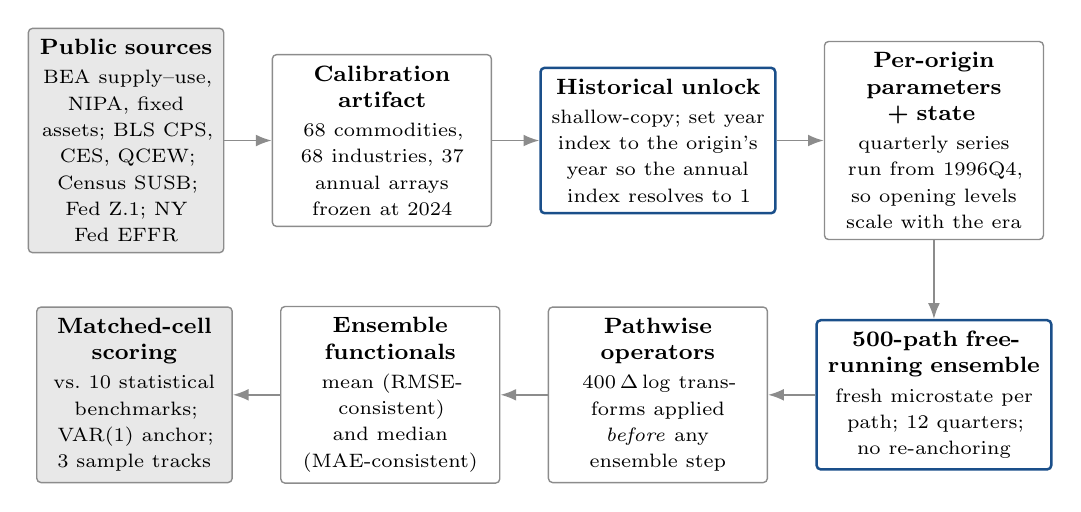
\begin{tikzpicture}[
  font=\footnotesize,
  node distance=6mm,
  box/.style={draw=greyrule,fill=white,rounded corners=1.5pt,align=center,
              inner sep=4pt,minimum height=8mm,text width=25mm,line width=0.5pt},
  data/.style={box,fill=greypale,text width=22mm},
  key/.style={box,draw=accent,line width=0.9pt,text width=27mm},
  ar/.style={-{Latex[length=2mm]},draw=greyrule,line width=0.6pt}
]
\node[data] (src)  {\textbf{Public sources}\\[1pt]\scriptsize BEA supply--use, NIPA,
                    fixed assets; BLS CPS, CES, QCEW; Census SUSB; Fed Z.1; NY Fed EFFR};
\node[box,right=of src] (cal) {\textbf{Calibration artifact}\\[1pt]\scriptsize 68 commodities,
                    68 industries, 37 annual arrays frozen at 2024};
\node[key,right=of cal] (unlock) {\textbf{Historical unlock}\\[1pt]\scriptsize shallow-copy;
                    set year index to the origin's year so the annual index resolves to 1};
\node[box,right=of unlock] (state) {\textbf{Per-origin\\parameters + state}\\[1pt]\scriptsize
                    quarterly series run from 1996Q4, so opening levels scale with the era};

\node[key,below=10mm of state] (ens) {\textbf{500-path free-running ensemble}\\[1pt]\scriptsize
                    fresh microstate per path; 12 quarters; no re-anchoring};
\node[box,left=of ens] (ops) {\textbf{Pathwise operators}\\[1pt]\scriptsize
                    $400\,\Delta\log$ transforms applied \emph{before} any ensemble step};
\node[box,left=of ops] (func) {\textbf{Ensemble functionals}\\[1pt]\scriptsize
                    mean (RMSE-consistent) and median (MAE-consistent)};
\node[data,left=of func] (score) {\textbf{Matched-cell scoring}\\[1pt]\scriptsize
                    vs.\ 10 statistical benchmarks; VAR(1) anchor; 3 sample tracks};

\draw[ar] (src) -- (cal);
\draw[ar] (cal) -- (unlock);
\draw[ar] (unlock) -- (state);
\draw[ar] (state) -- (ens);
\draw[ar] (ens) -- (ops);
\draw[ar] (ops) -- (func);
\draw[ar] (func) -- (score);
\end{tikzpicture}
\caption{\textbf{F7 --- the forecasting pipeline.} Public source data are compiled once into a
calibration artifact whose annual structural block is a single 2024 row. The historical unlock
re-points the annual index so that the artifact can be instantiated at any origin; the quarterly
series, which run from 1996Q4, then supply era-appropriate opening levels. Each origin is simulated
500 times, transformed pathwise, reduced to a mean and a median point forecast, and scored on
cells shared with every statistical benchmark.}
\label{fig:pipeline}
\end{figure}

\subsection{Operators}

Forecast targets are constructed \emph{pathwise, before any ensemble operation}. Writing $rg$ and
$ng$ for a path's real and nominal GDP series and taking row~1 as the origin, so that horizon $h$
is row $h+1$:
\begin{align}
\text{real\_gdp} &= 400\,\big(\log rg_{h+1} - \log rg_{h}\big), \\
\text{gdp\_deflator} &= 400\,\big[(\log ng_{h+1}-\log rg_{h+1}) - (\log ng_{h}-\log rg_{h})\big], \\
\text{nominal\_gdp} &= 400\,\big(\log ng_{h+1} - \log ng_{h}\big), \\
\text{EFFR} &= 100\,\big((1+r_{h+1})^4-1\big).
\end{align}
The \emph{GDP deflator} is the ratio of nominal to real GDP --- the economy-wide price index
implied by the accounts --- so its log difference is nominal growth minus real growth. Writing it
in log form rather than as a ratio is algebraically identical and finite for all positive
floating-point inputs. The quarterly-to-annual-rate scaling cancels from log differences, so
$400 = 4\times 100$ is the complete annualisation. Unemployment has no field in the data structure
and is read off agent state inside the stepping loop, with $H^{\mathrm{act}}=1\,826$ --- the
concept closest to the labour-force denominator --- in the denominator.

\subsection{Ensemble functionals}

Two point forecasts are emitted per cell, as separate model columns: the \emph{mean} of the
pathwise-transformed values and the \emph{median}. This follows \citet{gneiting2011}: the optimal
point forecast depends on the loss function, the mean being the Bayes act under squared error and
the median under absolute error. Reporting both is what allowed the first pass's mean-absolute-error
weakness to be attributed correctly (\S\ref{sec:v2}) instead of being blamed on the choice of
functional.

\subsection{The comparator field}

Fourteen model columns are scored: ten statistical benchmarks plus mean and median columns for each
of the two ABM versions. Table~\ref{tab:benchmarks} gives the specifications, taken from the
benchmark module's own type definitions.

\begin{table}[t]
\centering
\caption{The ten statistical benchmarks. All are estimated on training data only at each origin,
with hyperparameters fixed before the fit and encoded in the model identifier; none is tuned inside
the evaluation.}
\label{tab:benchmarks}
\small
\begin{tabular}{@{}rp{0.30\textwidth}p{0.51\textwidth}@{}}
\toprule
\# & \code{model_id} & Specification \\
\midrule
1 & \code{naive_no_change} & Random walk: forecast equals the last training observation. \\
2 & \code{naive_drift} & Random walk with drift estimated from training differences only. \\
3 & \code{naive_historical_mean} & Constant forecast equal to the training-sample mean. \\
4 & \code{univariate_ar_p1_constant} & Univariate AR(1) with intercept, per target. \\
5 & \code{univariate_ar_p4_constant} & Univariate AR(4) with intercept. \\
6 & \code{univariate_ar_bic_...} & Lag order chosen by the Bayesian information criterion on a
    common, training-only window. \\
7 & \code{beforeit_var_p1_constant} & Multivariate VAR(1) with intercept over the eight-target
    panel. \textbf{Ratio anchor.} \\
8 & \code{beforeit_var_p2_constant} & VAR(2). \\
9 & \code{beforeit_var_p3_constant} & VAR(3). \\
10 & \code{bvar_mniw_v1_p1_...} & Natural-conjugate Bayesian VAR with a matrix-normal /
    inverse-Wishart prior and Minnesota-style shrinkage \citep{litterman1986}: tightness 0.2, lag
    decay 1.0, own-lag prior mean 0.0, intercept variance 100, inverse-Wishart degrees-of-freedom
    offset 2, innovation scale 1.0, scale floor $10^{-8}$. \\
\bottomrule
\end{tabular}
\end{table}

The VAR(1) is the ratio anchor: every reported ratio is a model's score divided by the VAR(1)'s
score on the same cell, so values below 1.0 mean the model beats the anchor. The anchor is not a
strong benchmark --- at the 2010Q2 origin its estimated companion matrix has spectral radius 1.0342
and design condition number 8\,747, i.e.\ it is borderline explosive and poorly conditioned --- and
this should temper any reading of the absolute level of a ratio, though not of the differences
between models scored against the same anchor.

A fixed-parameter semi-structural state-space comparator (potential growth, output gap, natural
unemployment, neutral real rate, inflation anchor, inflation, policy rate and lagged output gap,
with a fixed transition encoding IS, Phillips, Okun and Taylor links, updated by an exact Kalman
filter) exists in the repository but is \emph{not} in this field: it scores a core-four target set
of which the ABM cannot serve the personal consumption expenditures price index. Its standing from
a separate 11-model comparison is a weighted RMSE ratio of 0.749 (1 of 11, all-available) and 0.745
(1 of 11, balanced), quoted as context only, on a different target set and a different field.

\subsection{Truth, scaling and score construction}

Truth is the revised panel itself; the error sign convention is forecast minus actual. Target
transformations are \emph{not} uniform across the panel: the four GDP-family series are
$400\ln(\text{level}_t/\text{level}_{t-1})$; the unemployment rate is a quarterly mean of three
monthly levels with no transform; EFFR is the equal-weight mean of published business-day rates
within the quarter \citep{ny_effr}.

Three scores are reported. \emph{RMSE} (root mean squared error) penalises large errors
quadratically; \emph{MAE} (mean absolute error) penalises them linearly; \emph{MASE} (mean absolute
scaled error, \citealp{hyndmankoehler2006}) divides MAE by the in-sample mean absolute first
difference of the same series, making it scale-free and directly comparable across targets. MASE
scales are recomputed at every origin from training data only.

The \emph{weighted ratio} used for the standings is a macro-average of matched cellwise ratios,
\begin{equation}
  \mathcal{W} \;=\; \sum_{\text{targets}}\sum_{h}\;
  w_{\text{target}}\; w_h \;\frac{\text{score}_{\text{model}}(\text{target},h)}
  {\text{score}_{\text{anchor}}(\text{target},h)},
  \qquad
  w_h \in \{0.30, 0.25, 0.20, 0.15, 0.10\},
\end{equation}
with equal target weights and horizon weights declining in $h$. It is explicitly \emph{not} a ratio
of pooled losses, which would let one badly scaled target dominate. A model is marked
\code{INCOMPLETE_MATCHED_GRID_NOT_RANKED} unless it has every target-by-horizon cell and zero
failures; every ABM column here is \code{COMPLETE_MATCHED} at 10 of 10 cells on all tracks and both
target sets.

The scoring key is (origin, target, horizon), and only cells where \emph{every} model in the field
is present survive. Because both ABM versions were scored in a single run, the version contrast
cannot be a sample artifact.

\subsection{Sample tracks and the pandemic mask}

\begin{table}[h]
\centering
\caption{The three sample tracks and their common-cell counts. The pandemic mask is applied to
\emph{target} periods, not origins, and was pre-registered in the run manifest rather than selected
after seeing results.}
\label{tab:tracks}
\small
\begin{tabular}{@{}llc@{}}
\toprule
Track & Rule & $n$ at $h=1/2/4/8/12$ \\
\midrule
all-available & every common cell & 61 / 60 / 58 / 54 / 50 \\
balanced $h{=}12$ & origins with a complete 12-quarter horizon & 50 / 50 / 50 / 50 / 50 \\
pandemic-masked & exclude cells whose target period falls in 2020Q1--2021Q4 & 53 / 52 / 50 / 46 / 42 \\
\bottomrule
\end{tabular}
\end{table}

\subsection{Monte-Carlo error}

The ABM's point forecast is an ensemble functional over finitely many stochastic paths, so its
measured RMSE is inflated by approximately $\sqrt{1+(\mathrm{se}_{\mathrm{MC}}/\mathrm{RMSE})^2}$.
Table~\ref{tab:mc} shows that at 500 paths this is negligible: against a real-GDP cross-origin RMSE
of order 6\pp, a Monte-Carlo standard error of 0.14\pp\ inflates the measured RMSE by well under
0.1\,\%. (At the 16-path pilot count the standard error was 1.3\pp\ and \emph{was} material; 500
paths were used precisely to remove the confound.)

\begin{table}[h]
\centering
\caption{Monte-Carlo error at 500 paths, ranges over the five horizons. ``Ensemble s.d.'' is the
dispersion of the simulated paths --- genuine model uncertainty; ``MC s.e.'' is the sampling error
of the ensemble mean --- simulation noise.}
\label{tab:mc}
\small
\begin{tabular}{@{}lccc@{}}
\toprule
Target & Mean ensemble s.d. & Mean MC s.e.\ of the mean & Max MC s.e. \\
\midrule
\code{real_gdp} & 3.036--3.269 & 0.136--0.146 & 0.255 \\
\code{gdp_deflator} & 0.860--1.077 & 0.038--0.048 & 0.100 \\
\code{nominal_gdp} & 3.211--3.440 & 0.144--0.154 & 0.264 \\
\code{unemployment_rate} & 0.414--1.079 & 0.019--0.048 & 0.070 \\
\code{effective_federal_funds_rate} & 0.139--0.336 & 0.006--0.015 & 0.019 \\
\bottomrule
\end{tabular}
\end{table}

\subsection{The opening-row measurement basis}

One artifact of initialisation must be declared because it affects the $h=1$ cell, which carries
the largest horizon weight. The initialiser writes row~1 on a different measurement basis from
rows~2 onwards: prices are normalised to 1 at initialisation, so real and nominal GDP coincide in
row~1 and the model-implied opening deflator is exactly 1.0. The opening row is the
\emph{model-implied} opening, not an observed control --- reassuring for leakage, unhelpful for
$h=1$ comparability. Dropping $h=1$ was rejected outright: it would render the grid incomplete and
the model unranked. It is reported and flagged.

% ===========================================================================
\section{Results I: the first pass}
\label{sec:v1}

All results in \S\ref{sec:v1}--\S\ref{sec:v2} are computed from the joint scoring run in which both
ABM columns were scored together on identical cells. The first-pass column reproduced the earlier
standalone run bit-identically over all 3\,660 cached cells (gate G4 in
Table~\ref{tab:gates}).

\subsection{Standings}

\begin{table}[h]
\centering
\caption{First-pass (\code{v1}) standings on the headline target pair \{real GDP growth,
GDP-deflator inflation\}. Ranks are out of the 14 scored forecast columns.}
\label{tab:v1standings}
\small
\begin{tabular}{@{}lccl@{}}
\toprule
Track & v1 mean ratio (rank) & v1 median ratio (rank) & Best statistical \\
\midrule
all-available & 0.905 (5th) & 0.903 (4th) & \code{naive_historical_mean} 0.879 \\
balanced $h{=}12$ & 0.894 (5th) & 0.893 (4th) & \code{naive_historical_mean} 0.884 \\
pandemic-masked & 1.272 (11th) & 1.264 (10th) & \code{univariate_ar_p1} 0.848 \\
\bottomrule
\end{tabular}
\end{table}

Competitive on the first two tracks --- and eleventh of fourteen once the COVID cells are removed.
That regime dependence was, at the time, the most alarming feature of the result: a model whose
standing depends on the presence of the two most anomalous years in the sample is not obviously
forecasting anything.

\subsection{The bias}

Table~\ref{tab:percell} (\S\ref{sec:v2}, left-hand columns) gives the detail. Real GDP growth is
under-forecast by $-1.32$, $-7.28$, $-2.94$, $-2.15$ and $-2.02$\pp\ at $h=1,2,4,8,12$. The
$-7.28$\pp\ figure at $h=2$ is a transient; the $-2$ to $-3$\pp\ figures at the longer horizons are
a chronic level bias. The deflator, by contrast, was already the strongest headline target, with
ratios of 0.771--0.975 at every horizon and MAE ratios uniformly below one.

\subsection{The mean-absolute-error asymmetry}

The first pass's headline RMSE ratio of 0.905 sat against an MAE ratio of 1.137 --- it beat the
anchor under quadratic loss and lost under linear loss. Disaggregating shows the asymmetry was
never general: on the deflator and the policy rate the MAE ratios were already below one. It was
concentrated in real and nominal GDP and, within those, in the $h=2$ cell (MAE ratios 2.376 and
2.071 respectively). Switching to the loss-consistent median improved the weighted MAE ratio only
from 1.137 to 1.130, so it was \emph{not} a functional-choice artifact.

\subsection{Burn-in: a negative result, retained}

Burn-in --- building the model $k$ quarters before the origin and treating row $k+1$ as the origin
--- was the leading candidate fix for the $h=2$ transient. It was tried at $k=1$ and $k=4$ with 128
paths, and it failed in an instructive way. One quarter of burn-in \emph{relocates} the transient
from $h=2$ to $h=1$, where the horizon weight is larger, so the weighted result worsens (0.905
$\rightarrow$ 0.954). Four quarters disperses the transient (headline MAE ratio improves to 1.012)
but destroys the level targets: the policy-rate $h=1$ ratio degrades from 0.563 to 2.091 and the
secondary weighted ratio from 0.782 to 1.095, because four quarters of free-running drift move the
model's policy rate away from the origin's observed level before scoring begins. Burn-in trades a
growth-rate artifact for a level-drift information loss.

This entire line of attack is moot after the repair --- the $h=2$ bias falls to $-0.096$\pp\ under
the balance fix alone, with zero burn-in --- and the burn-in runs are retained only as documented
negative results.

% ===========================================================================
\FloatBarrier
\section{Diagnosis: the anatomy of a \texorpdfstring{$-2.75$}{-2.75} percentage-point bias}
\label{sec:diagnosis}

This section rests on matched-seed A/B experiments at four to five origins with 48--64 paths per
cell, with seeds identical across every variant. The bias measured here is $h=3\ldots12$ annualised
real GDP growth, ensemble mean minus realised, averaged over three clean origins (2012Q4, 2016Q4,
2022Q4; 2019Q4 is excluded from every average because its window is the pandemic rebound at
$+6.2$\pp). The baseline is $-2.750$\pp, consistent with the $-2.0$ to $-2.9$\pp\ per-horizon biases
measured independently at 61 origins.

\subsection{Ranked attribution}

\begin{table}[h]
\centering
\caption{Ranked attribution of the $-2.75$\pp\ real-growth bias.}
\label{tab:attribution}
\small
\footnotesize
\begin{tabular}{@{}r>{\raggedright\arraybackslash}p{0.43\textwidth}r>{\raggedright\arraybackslash}p{0.21\textwidth}@{}}
\toprule
\# & Mechanism & Share & Confidence \\
\midrule
1 & Non-clearing sector commodity balance under explicit measured trade, colliding with a frozen
    firm capacity envelope & $-2.10$\pp\ (76\,\%) & high \\
2 & Growth expectation from an OLS AR(1) on log levels, delivering 32--63\,\% of the in-sample
    trend & $-0.70$\pp\ (24\,\%) & high (estimator), medium (delivered size) \\
3 & Opening inventories built from the negative half of a signed statistical discrepancy
  & $-0.23$\pp\ (a subset of \#1) & high \\
4 & No capital accumulation (replacement-only investment) & latent; binds only through \#1 & high \\
5 & Exogenous government/export/import log-level AR(1) attractors & $\approx 0$ net & high \\
\bottomrule
\end{tabular}
\end{table}

The GDP deflator is untouched throughout --- 1.8--2.5\,\% in every variant --- which is why
inflation was never biased. \textbf{The defect is a real quantity-rationing defect, not a pricing
defect.} \S\ref{sec:v2} confirms this prediction out of sample.

\subsection{The shortfall is broad-based}

Decomposing the expenditure side (contribution gap $=$ opening nominal share $\times$ (model $-$
realised)) shows every domestic component growing at 0.1--0.5\,\% annualised against realised
2.5--5.4\,\%:

\begin{table}[h]
\centering
\caption{Expenditure decomposition, $h=3\ldots12$ annualised; contribution gaps in percentage
points of GDP growth. Consumption carries $\approx70\,\%$ of the gap and fixed investment
$\approx25\,\%$ \emph{purely because of their weights} --- their growth rates are equally flat
(0.11--0.36\,\%). Net trade contributes positively; exports are over-forecast by 1.3--3.0\pp.}
\label{tab:expenditure}
\small
\begin{tabular}{@{}lrrrrrr@{}}
\toprule
Origin & $C$ & $I$ fixed & $G$ & $X$ & $M$ ($-$) & \textbf{GDP} \\
\midrule
2012Q4 & $-1.77$ & $-0.91$ & $-0.02$ & $+0.23$ & $+0.44$ & $\mathbf{-2.03}$ \\
2014Q4 & $-1.54$ & $-0.64$ & $-0.17$ & $+0.10$ & $+0.46$ & $\mathbf{-1.80}$ \\
2016Q4 & $-1.54$ & $-0.60$ & $-0.46$ & $+0.12$ & $+0.19$ & $\mathbf{-2.30}$ \\
2022Q4 & $-1.72$ & $-0.44$ & $-0.30$ & $-0.05$ & $+0.30$ & $\mathbf{-2.20}$ \\
\bottomrule
\end{tabular}
\end{table}

At the 68-sector level, 31--36 of 68 sectors show positive growth, and \emph{the same sectors lose
at every origin} --- the persistent-loser list is identical at 2012Q4, 2016Q4 and 2024Q4. A stable
loser set across twelve years of origins is a calibration signature, not a shock response.

\subsection{Defect 1: the commodity balance does not clear}
\label{sec:defect1}

Because imports come from the measured BEA T262 matrix rather than being solved as the supply--use
residual, the residual survives as a signed, sector-level gap. Measured on the shipped first-pass
artifact:
\begin{gather*}
\frac{\text{aggregate uses}}{\text{aggregate supply}} = 1.01010, \\[2pt]
\min -0.706 \;\mid\; p_{25}\, -0.058 \;\mid\; \text{med.} +0.020 \;\mid\;
p_{75}\, +0.128 \;\mid\; \max +0.476,
\end{gather*}
with 42 of 68 commodities over-demanded, 34 with $|\text{gap}|>10\,\%$ and 8 with
$|\text{gap}|>25\,\%$ (mean $|\text{gap}|$ 0.1262, standard deviation 0.1790). The left panel of
Figure~\ref{fig:balance} shows the distribution.

Two facts then lock the chain, and Figure~\ref{fig:mechanism} draws it.

\begin{enumerate}[leftmargin=1.6em,itemsep=2pt]
\item \textbf{The capacity envelope is fixed by construction.} $\omega=0.85$ is hard-coded, and the
  capital calibration gives $K_i\kappa_i = Y_i/0.85$ identically, so every firm opens at exactly
  85\,\% utilisation with 17.6\,\% headroom, in proportion to the \emph{opening output}
  composition.
\item \textbf{Capital never accumulates.} Replacement-only investment gives $K'=K$ exactly when
  firms obtain desired investment and produce at target. Measured $K_{\text{end}}/K_1 =
  1.0000$--$1.0009$ in every variant, \emph{including} under a 30\,\% capacity relief.
\end{enumerate}

The demand vector, meanwhile, is fixed by the coefficient matrices, and the two differ by exactly
the 42/26 signed gap. Over-demanded sectors sit permanently against their ceiling, under-demanded
ones permanently idle, and the $\min$ in Eq.~\eqref{eq:leontief} is one-sided so the idle capacity
never compensates. The signature matches the mechanism precisely:

\begin{itemize}[leftmargin=1.4em,itemsep=1pt]
\item mean $(\text{uses}-\text{supply})/\text{supply}$ of the twelve most-truncated sectors is
      $+0.222$, against $+0.014$ for all 68;
\item mean gap of the persistent value-added losers is $-0.140$, against $-0.025$ for the winners;
\item 46 of 68 sectors are \emph{never} truncated, while a stable minority is truncated in
      40--80\,\% of quarters;
\item 12.9--14.4\,\% of gross output is produced under a binding ceiling every quarter, at
      every origin tested (Table~\ref{tab:doseresponse}, last column).
\end{itemize}

Downstream, the unmet demand appears as persistent rationing, stable at every horizon:

\begin{table}[h]
\centering
\caption{Fill rates --- the fraction of each buyer's demand actually satisfied --- in the
first-pass model. Exports are the worst-served buyer because the export basket is concentrated in
over-demanded commodities. Relieving opening capacity by 30\,\% lifts the export fill rate to
0.92--0.96, which establishes that export rationing is a \emph{symptom} of the capacity/balance
collision rather than an independent trade defect.}
\label{tab:fillrates}
\small
\begin{tabular}{@{}lccccc@{}}
\toprule
Fill rate & $h=1$ & $h=2$ & $h=4$ & $h=8$ & $h=12$ \\
\midrule
Households & 0.999 & 0.973 & 0.978 & 0.976 & 0.975 \\
Government & 0.999 & 0.961 & 0.961 & 0.960 & 0.958 \\
\textbf{Exports} & 0.995 & \textbf{0.845} & \textbf{0.869} & \textbf{0.865} & \textbf{0.862} \\
Imports & 0.993 & 0.991 & 0.989 & 0.989 & 0.987 \\
\bottomrule
\end{tabular}
\end{table}

\begin{figure}[t]
\centering
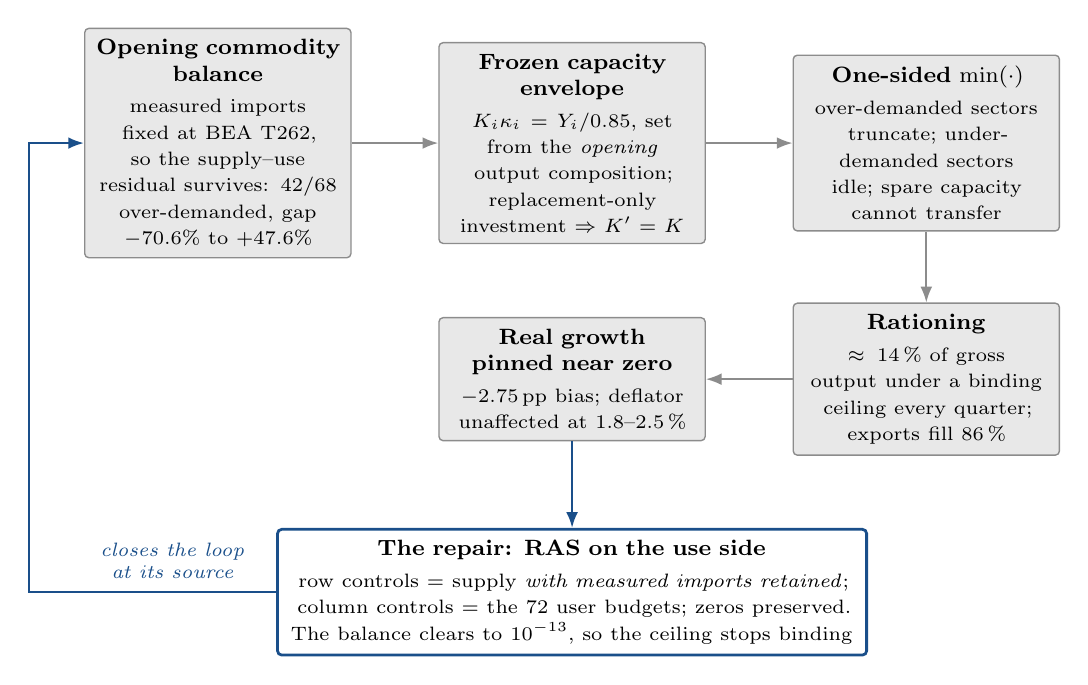
\begin{tikzpicture}[
  font=\footnotesize,
  box/.style={draw=greyrule,fill=white,rounded corners=1.5pt,align=center,
              inner sep=4pt,text width=31mm,line width=0.5pt},
  bad/.style={box,draw=greyrule,fill=greypale},
  fix/.style={box,draw=accent,line width=1.0pt,text width=72mm},
  ar/.style={-{Latex[length=2mm]},draw=greyrule,line width=0.7pt},
  arfix/.style={-{Latex[length=2mm]},draw=accent,line width=0.9pt}
]
\node[bad] (gap) {\textbf{Opening commodity\\balance}\\[2pt]\scriptsize
  measured imports fixed at BEA T262, so the supply--use residual survives:
  42/68 over-demanded, gap $-70.6\%$ to $+47.6\%$};
\node[bad,right=11mm of gap] (cap) {\textbf{Frozen capacity\\envelope}\\[2pt]\scriptsize
  $K_i\kappa_i = Y_i/0.85$, set from the \emph{opening} output composition;
  replacement-only investment $\Rightarrow K'=K$};
\node[bad,right=11mm of cap] (trunc) {\textbf{One-sided $\min(\cdot)$}\\[2pt]\scriptsize
  over-demanded sectors truncate; under-demanded sectors idle;
  spare capacity cannot transfer};
\node[bad,below=9mm of trunc] (ration) {\textbf{Rationing}\\[2pt]\scriptsize
  $\approx14\,\%$ of gross output under a binding ceiling every quarter; exports fill 86\,\%};
\node[bad,left=11mm of ration] (bias) {\textbf{Real growth pinned near zero}\\[2pt]\scriptsize
  $-2.75$\pp\ bias; deflator unaffected at 1.8--2.5\,\%};
\node[fix,below=11mm of bias] (ras) {\textbf{The repair: RAS on the use side}\\[2pt]\scriptsize
  row controls $=$ supply \emph{with measured imports retained}; column controls $=$ the 72
  user budgets; zeros preserved. The balance clears to $10^{-13}$, so the ceiling stops binding};

\draw[ar] (gap) -- (cap);
\draw[ar] (cap) -- (trunc);
\draw[ar] (trunc) -- (ration);
\draw[ar] (ration) -- (bias);
\draw[arfix] (bias) -- (ras);
\coordinate (L) at ([xshift=-7mm]gap.west);
\draw[arfix] (ras.west)
  -- node[above=1pt,pos=0.42,text=accent,font=\scriptsize\itshape,align=center]
     {closes the loop\\at its source} (L |- ras.west)
  -- (L) -- (gap.west);
\end{tikzpicture}
\caption{\textbf{F8 --- the defect mechanism and its repair.} Grey: the causal chain from a
non-clearing opening balance to a real-growth bias. Blue: the reconciliation closes the loop at its
source, by making the opening balance clear commodity by commodity while retaining every measured
import level. Because capacity relief and balance closure were shown to be \emph{substitutes}
rather than complements (Table~\ref{tab:falsification}), intervening at the balance is sufficient;
the frozen capacity envelope is left untouched.}
\label{fig:mechanism}
\end{figure}

\subsection{Defect 2: the growth expectation is biased low by construction}

The second defect is the estimator of Eq.~\eqref{eq:gammae} and Table~\ref{tab:gammae}. What makes
it interesting is that it is \emph{latent}. Replacing the model's opening output history by its own
log-linear trend --- a past-only intervention --- raises $\gamma_e$ from $\approx 1.0\,\%$ to
$\approx 1.9\,\%$ but moves delivered GDP growth by $+0.06$\pp\ on average. Pushing the expectation
to twice trend still delivers between $-0.06$ and $+0.04$\pp. The elasticity of delivered growth to
$\gamma_e$ is $\approx 0$ while the imbalance is present, rises to $\approx +0.5$\pp\ once capacity
headroom is opened, and reaches $+0.75$\pp\ once the balance is closed. Measured on the actual
patched code with 64 matched-seed paths at four origins, the random-walk-drift change is worth
$+0.193$\pp\ on the unreconciled baseline and $+0.499$\pp\ on the reconciled one --- the monotone
pattern the diagnosis predicted. \textbf{Expectations are a real but strictly subordinate defect:
fixing them is worth $+0.75$\pp, but only after fixing the balance.}

\subsection{The falsification table}

Each row of Table~\ref{tab:falsification} is a matched-seed experiment run to kill a competing
hypothesis. The sixth row is the decisive discriminator: capacity relief and balance closure are
\emph{substitutes}, not complements, which places the balance upstream.

\begin{table}[t]
\centering
\caption{Falsification experiments. All matched-seed, all at scale $10^{-5}$ unless stated.}
\label{tab:falsification}
\footnotesize
\begin{tabular}{@{}p{0.31\textwidth}p{0.30\textwidth}p{0.33\textwidth}@{}}
\toprule
Test & Result & Rules out \\
\midrule
Agent-count sweep, $130\rightarrow294\rightarrow912\rightarrow2\,708$ firms
& truncated share 14\,\% at \emph{every} scale; growth stays $\approx 0$
& idiosyncratic small-sample lumpiness \\
Materials-only relief, $M\times1.30$
& $-0.06$ against $-0.08$ baseline: no effect
& materials as an independent binding constraint \\
Investment-demand cut, $\kappa_s\times1.30$ (cuts $I^d$ by 23\,\%, leaves $K\kappa$)
& $-0.20$ against $-0.08$: $-0.12$\pp\ only
& investment demand as a first-order channel \\
Capacity tightening, $K\kappa\times0.77$
& $-1.14$ / $-1.22$\pp
& --- confirms the sign and convexity of the capacity margin \\
Un-capped investment emulation
& $-0.03$ against $-0.08$; $K_{\text{end}}/K_1=1.0005$
& ``the fork's $\min$ broke investment'' \\
\textbf{Legacy residual closure $+\;K\times1.30$}
& \textbf{1.921 vs 1.879 (2016Q4); 2.505 vs 2.503 (2024Q4): $+0.00$\pp}
& \textbf{capacity as an \emph{independent} cause} \\
Drop opening inventories only
& $+0.23$\pp\ mean, same sign at all four origins
& --- a genuine but small independent contribution \\
Labour-supply ceiling
& labour binds in 0.000 of rows at every origin
& the labour block as the constraint \\
Post-origin look-ahead in the exogenous arrays
& bit-identical paths under $-10^{99}$ poisoning
& data leakage \\
\bottomrule
\end{tabular}
\end{table}

\subsection{The dose--response that motivated the repair}

Reverting to the legacy residual closure --- solving imports as the supply--use residual, which
\emph{guarantees} clearing but discards the measured BEA import levels --- gives, for $h=3\ldots12$
annualised real GDP growth:

\begin{table}[h]
\centering
\caption{Dose--response. The legacy residual closure is a \emph{diagnostic instrument}, not the
shipped repair: it discards measured import levels. The shipped repair achieves exact clearing
while retaining them.}
\label{tab:doseresponse}
\small
\footnotesize
\begin{tabular}{@{}lrrrrl@{}}
\toprule
Origin & Realised & Baseline & Legacy closure & $+$ trend exp. & Truncated share \\
\midrule
2012Q4 & \textbf{2.586} & 0.051 & \textbf{2.365} & 3.511 & $0.144\rightarrow0.006$ \\
2016Q4 & \textbf{2.922} & $-0.079$ & \textbf{1.879} & 2.633 & $0.139\rightarrow0.002$ \\
2022Q4 & \textbf{2.531} & $-0.207$ & \textbf{1.813} & 2.458 & $0.129\rightarrow0.004$ \\
2024Q4 & --- & $-0.219$ & \textbf{2.503} & 2.623 & $0.143\rightarrow0.012$ \\
\midrule
\multicolumn{6}{@{}l}{Mean bias over the three clean origins:
$-2.76$\pp\ $\rightarrow$ $-0.66$\pp\ $\rightarrow$ $+0.19$\pp, deflator unchanged throughout.} \\
\bottomrule
\end{tabular}
\end{table}

% ===========================================================================
\FloatBarrier
\section{The repair}
\label{sec:repair}

Two changes, both in the calibration artifact rather than in behavioural parameters.

\subsection{(i) The opening commodity balance now clears}

A \emph{biproportional} adjustment --- the RAS method of \citet{stone1961} and
\citet{bacharach1970}, equivalently the minimum-$I$-divergence projection --- finds the matrix
closest to a given one, in a relative-entropy sense, subject to prescribed row and column totals. It
does so by alternately scaling rows and columns until both sets of margins are satisfied.

Formally, let $U^{0}\in\mathbb{R}_{\ge0}^{G\times J}$ be the observed use matrix over $G=68$
commodities and $J=72$ users (68 industry intermediate columns plus $C$, $G$, $I$ and $X$). We seek
\begin{equation}
  U^{\star} \;=\; \arg\min_{U\ge 0}\;\sum_{g,j} U_{gj}\log\frac{U_{gj}}{U^{0}_{gj}}
  \quad\text{s.t.}\quad
  \sum_j U_{gj} = r_g \;\;\forall g,
  \qquad \sum_g U_{gj} = c_j \;\;\forall j,
  \label{eq:ras}
\end{equation}
with row controls $r_g = \text{industry output}_g + \text{measured imports}_g$ and column controls
$c_j$ the 68 industry intermediate budgets and the four final-demand budgets. The solution has the
biproductive form $U^{\star}_{gj}=\rho_g\, U^{0}_{gj}\, s_j$ and is obtained by iterative
proportional fitting; structural zeros are preserved exactly, because a zero cell stays zero under
any scaling.

The concrete run is reported in Table~\ref{tab:ras}. Crucially, \code{use_explicit_trade} stays
\code{true}: no measured import level is discarded. The reconciliation works \emph{around} the
measured trade data rather than throwing it away, which is what distinguishes the shipped repair
from the legacy-closure diagnostic instrument of Table~\ref{tab:doseresponse}.

\begin{table}[h]
\centering
\caption{The RAS reconciliation as executed, from the committed reconciliation report. The
adjustment moves composition, not aggregates: every column budget is preserved to
$10^{-13}$ after the $\lambda$ scaling.}
\label{tab:ras}
\small
\footnotesize
\begin{tabular}{@{}p{0.34\textwidth}>{\raggedright\arraybackslash}p{0.58\textwidth}@{}}
\toprule
Flow system & 68 commodities $\times$ 72 users \\
Structural zeros preserved & 1\,549 / 4\,896 cells (31.6\,\%) \\
Row controls & $\text{industry output} + \text{measured imports}$, sum $5.25699\times10^{7}$ \\
Column controls & measured budgets, held exactly, sum $5.25699\times10^{7}$ \\
Convergence & 623 iterations; final max relative control error $9.996\times10^{-14}$ \\
Balance after RAS & $\max|\text{uses}_g/\text{supply}_g-1| = 5.55\times10^{-16}$;
                    cross-sector s.d.\ $1.96\times10^{-16}$ (was 0.1790) \\
Balance after re-derivation & $\max|\text{uses}_g/\text{supply}_g-1| = 1.00\times10^{-13}$ \\
Total use adjustment & $\sum|d| = 6.786\times10^{6}$ (12.78\,\% of total uses) \\
Cellwise adjustment & $\sum|dU| = 7.423\times10^{6}$ (13.98\,\% of total flow) \\
\midrule
\multicolumn{2}{@{}l}{\emph{Coefficient movement received by the simulator}} \\
Technology matrix $a_{sg}$ & $\max|\Delta a| = 0.1408$; mean $|\Delta a| = 0.00226$ \\
Household basket $b^{HH}_g$ & $\max|\Delta\text{share}| = 0.0158$; $L_1$ distance 0.0970 \\
Government basket $c^{G}_g$ & $\max|\Delta\text{share}| = 0.1450$; $L_1$ distance 0.3204 \\
Investment basket $b^{CF}_g$ & $\max|\Delta\text{share}| = 0.0401$; $L_1$ distance 0.1049 \\
Export basket $c^{E}_g$ & $\max|\Delta\text{share}| = 0.0309$; $L_1$ distance 0.1197 \\
Import basket $c^{I}_g$ & unchanged \\
\bottomrule
\end{tabular}
\end{table}

The adjustment is not uniform across users: as a share of its own budget, the government column
moves most (31.0\,\%), then intermediates (15.3\,\%), exports (12.1\,\%), investment (10.0\,\%) and
households (9.8\,\%). The largest single commodity adjustments are professional and technical
services (uses cut 32.3\,\%, closing a $+47.6\,\%$ gap), wholesale trade (raised 42.5\,\%, closing a
$-29.8\,\%$ gap) and state and local government (raised 26.2\,\%). Figure~\ref{fig:balance} shows
the before-and-after distribution.

The one accounting choice --- production-account anchoring by $\lambda=0.983460$ --- is stated in
assumption A6 and Table~\ref{tab:lambda}, and its semantics are sealed verbatim in every result
manifest.

\begin{figure}[t]
\centering
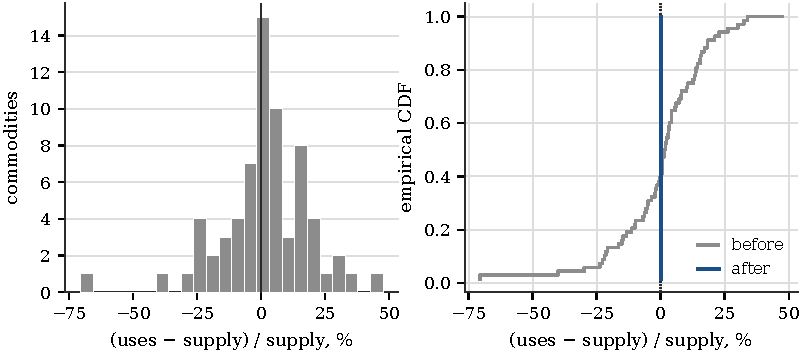
\includegraphics[width=\textwidth]{figures/f5_commodity_balance.pdf}
\caption{\textbf{F5 --- the opening commodity balance, before and after reconciliation.} Left: the
distribution of $(\text{uses}_g-\text{supply}_g)/\text{supply}_g$ over the 68 commodities of the
first-pass artifact, spanning $-70.6\,\%$ to $+47.6\,\%$ with a standard deviation of 17.9
percentage points. Right: the empirical cumulative distribution before (grey) and after (blue). The
post-reconciliation distribution is a step function at zero: every commodity clears to within
$10^{-13}$. Data: \code{reconciliation_by_commodity_rho1.csv}.}
\label{fig:balance}
\end{figure}

\subsection{(ii) Growth expectations become a random walk with drift}

The repaired model pins $\hat\alpha=1$ and takes the drift as average past log growth --- the
correctly specified estimator for an I(1)-with-drift series, on past data only. It is gated behind
a new model property, registered only when the calibration artifact carries the corresponding
marker, and \emph{default-off}, so the Austrian and Italian calibrations remain bit-identical
(gate G3). Exactly one Normal variate is consumed on either branch, which keeps the matched-seed
comparison aligned.

\subsection{Regression gates}

\begin{table}[t]
\centering
\caption{Regression gates on the repair. G7 is a pre-existing repository-wide formatter failure on
files untouched by this work, tracked separately. G8 is reported as failing on the merits rather
than hidden.}
\label{tab:gates}
\footnotesize
\begin{tabular}{@{}rp{0.24\textwidth}p{0.60\textwidth}@{}}
\toprule
\# & Gate & Result \\
\midrule
G1 & matched-grid completeness
   & \textbf{PASS} --- 61/61 origins; counts $[61,60,58,54,50]$, $[50,50,50,50,50]$,
     $[53,52,50,46,42]$; every ABM column \code{COMPLETE_MATCHED} \\
G2 & no non-finite output
   & \textbf{PASS} --- 0 non-finite cells in $3\,660+3\,660+120$ ensemble rows;
     500 paths used at every origin; 0 failed; the failures file is empty \\
G3 & Austria/Italy unchanged with the flag off
   & \textbf{PASS} --- 3 seeds $\times$ 3 series, SHA-256 of raw \code{Float64} vectors identical
     between a pristine checkout and the patched worktree \\
G4 & first-pass column reproduces its own earlier run
   & \textbf{PASS} --- all 3\,660 cached cells identical ($\max|\text{diff}|=0$); weighted scores
     match to every printed digit \\
G5 & GDP-deflator inflation stays $\approx2\,\%$
   & \textbf{PASS} --- 2.019\pp\ (p5 1.663, p95 2.687) against 2.024\pp\ over the same 671 scored
     cells; \emph{bit-identical at $h=1$} \\
G6 & commodity balance clears in the shipped artifact
   & \textbf{PASS} --- $1.0\times10^{-13}$ after re-derivation through the unmodified pipeline \\
G7 & package test suite
   & \textbf{PARTIAL} --- 815 pass, 1 fail; the failure is a repository-wide formatter check that
     already failed at the base commit on ten files untouched here \\
G8 & unemployment
   & \textbf{REPORTED, FAILING ON MERIT} --- \S\ref{sec:unemployment} \\
\bottomrule
\end{tabular}
\end{table}

% ===========================================================================
\FloatBarrier
\section{Results II: the repaired model}
\label{sec:v2}

\subsection{Standings: first of fourteen in all three tracks}

\begin{table}[t]
\centering
\caption{Headline standings, \{real GDP growth, GDP-deflator inflation\}, \emph{all-available}
track ($n = 61/60/58/54/50$). Ratios are weighted macro-averages of matched cellwise ratios against
the VAR(1) anchor; lower is better. First-pass rows are italicised.}
\label{tab:standings}
\small
\begin{tabular}{@{}rlrr@{}}
\toprule
Rank & Model & Weighted RMSE ratio & Weighted MAE ratio \\
\midrule
\textbf{1} & \textbf{ABM v2, mean} & \textbf{0.830} & \textbf{0.813} \\
\textbf{2} & \textbf{ABM v2, median} & \textbf{0.830} & \textbf{0.815} \\
3 & \code{naive_historical_mean} & 0.879 & 0.838 \\
4 & \emph{ABM v1, median} & \emph{0.903} & \emph{1.130} \\
5 & \emph{ABM v1, mean} & \emph{0.905} & \emph{1.137} \\
6 & \code{bvar_mniw_v1_p1_constant} & 0.908 & 0.896 \\
7 & \code{univariate_ar_p1_constant} & 0.918 & 0.888 \\
8 & \code{univariate_ar_bic_...} & 0.929 & 0.901 \\
9 & \code{univariate_ar_p4_constant} & 0.939 & 0.923 \\
10 & \code{beforeit_var_p1_constant} (anchor) & 1.000 & 1.000 \\
11 & \code{naive_no_change} & 1.075 & 1.121 \\
12 & \code{naive_drift} & 1.106 & 1.156 \\
13 & \code{beforeit_var_p2_constant} & 2.121 & 1.496 \\
14 & \code{beforeit_var_p3_constant} & 5.313 & 2.672 \\
\bottomrule
\end{tabular}
\end{table}

On the \emph{balanced $h{=}12$} track ($n=50$ everywhere) the repaired mean column scores 0.829
(1st), its median 0.830 (2nd), \code{naive_historical_mean} 0.884 (3rd), the first-pass columns
0.893 and 0.894 (4th, 5th), and the BVAR 0.909 (6th).

On the \emph{pandemic-masked} track ($n=53/52/50/46/42$) the repaired mean column scores 0.796
(1st) and its median 0.799 (2nd), ahead of \code{univariate_ar_p1} at 0.848, the BVAR at 0.852,
\code{univariate_ar_bic} at 0.870, \code{naive_historical_mean} at 0.881 and
\code{univariate_ar_p4} at 0.889; the first-pass columns fall to 1.264 and 1.272 (10th, 11th).

\begin{figure}[t]
\centering
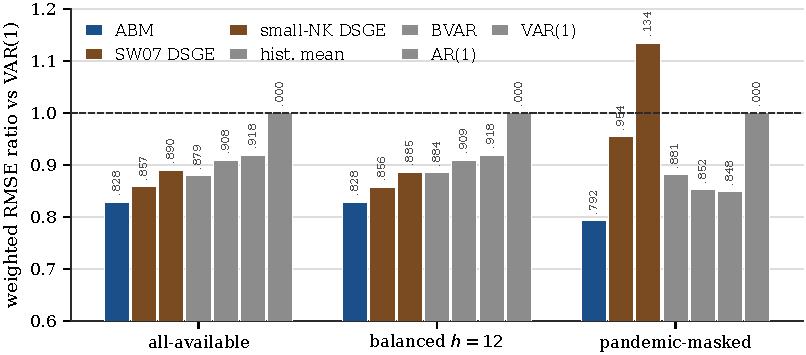
\includegraphics[width=\textwidth]{figures/f1_weighted_rmse_ratio.pdf}
\caption{\textbf{F1 --- weighted RMSE ratio on the headline target pair, three sample tracks.}
Blue is the repaired ABM; hatched pale blue is the first pass; greys are statistical benchmarks. The
dashed line is the VAR(1) anchor at 1.0. The repaired model is first in all three tracks, and its
margin is \emph{widest} in the pandemic-masked sample --- the opposite of the first pass's
behaviour. Data: \code{weighted_relative_scores.csv}.}
\label{fig:f1}
\end{figure}

\textbf{The regime-sensitivity finding resolves in the repaired model's favour.} The first pass's
competitive rank \emph{depended} on the COVID cells: masking 2020Q1--2021Q4 moved it from 5th
(0.905) to 11th (1.272). The repaired model carries no such dependence --- it is 1st in the masked
sample and by its \emph{widest} margin (0.796 against 0.848 for the best statistical model, a
6.1\,\% gap, against 5.6\,\% all-available). The regime sensitivity was a symptom of the defect: in
the calm sample the chronic $-2$\pp\ bias dominated the error, while in the full sample it was
partly hidden by cells that no model forecasts. Removing the bias removes the sensitivity.

\subsection{Per-cell detail}

\begin{table}[t]
\centering
\caption{Per-target, per-horizon detail, \emph{all-available} track. Ratios are against the VAR(1)
anchor; ranks are out of the 14 scored forecast columns. Bias is the mean error (forecast $-$ realised) in annualised
percentage points. Read the last two columns together: the repair removes a chronic level bias
without touching the price block.}
\label{tab:percell}
\footnotesize
\begin{tabular}{@{}llrrrrrccrr@{}}
\toprule
Target & $h$ & $n$ & v1 RMSE & v2 RMSE & v1 ratio & v2 ratio & v1 rank & v2 rank & v1 bias & \textbf{v2 bias} \\
\midrule
\code{real_gdp} & 1 & 61 & 6.2592 & 6.0879 & 0.689 & \textbf{0.670} & 4/14 & \textbf{1/14} & $-1.317$ & $\mathbf{-0.025}$ \\
\code{real_gdp} & 2 & 60 & 9.5104 & 6.1001 & 1.294 & \textbf{0.830} & 12/14 & \textbf{1/14} & $-7.277$ & $\mathbf{-0.096}$ \\
\code{real_gdp} & 4 & 58 & 6.8762 & 6.2235 & 1.082 & 0.980 & 8/14 & 3/14 & $-2.938$ & $\mathbf{-0.143}$ \\
\code{real_gdp} & 8 & 54 & 6.7381 & 6.4418 & 0.858 & 0.820 & 8/14 & 3/14 & $-2.146$ & $\mathbf{-0.119}$ \\
\code{real_gdp} & 12 & 50 & 6.9637 & 6.6510 & 1.035 & 0.988 & 10/14 & 3/14 & $-2.017$ & $\mathbf{-0.202}$ \\
\addlinespace
\code{gdp_deflator} & 1 & 61 & 1.4288 & 1.4288 & 0.794 & 0.794 & 6/14 & 5/14 & $-0.192$ & $-0.192$ \\
\code{gdp_deflator} & 2 & 60 & 1.6486 & 1.6544 & 0.771 & 0.774 & 5/14 & 8/14 & $-0.293$ & $-0.292$ \\
\code{gdp_deflator} & 4 & 58 & 1.9398 & 1.9512 & 0.822 & 0.827 & 2/14 & 6/14 & $-0.400$ & $-0.421$ \\
\code{gdp_deflator} & 8 & 54 & 2.0391 & 2.0448 & 0.975 & 0.978 & 4/14 & 5/14 & $-0.525$ & $-0.528$ \\
\code{gdp_deflator} & 12 & 50 & 2.1093 & 2.1080 & 0.892 & 0.891 & 5/14 & 4/14 & $-0.608$ & $-0.615$ \\
\addlinespace
\code{nominal_gdp} & 1 & 61 & 7.0266 & 6.8395 & 0.674 & \textbf{0.656} & 4/14 & \textbf{1/14} & $-1.509$ & $-0.217$ \\
\code{nominal_gdp} & 2 & 60 & 10.1803 & 6.7821 & 1.168 & \textbf{0.778} & 12/14 & \textbf{1/14} & $-7.569$ & $-0.388$ \\
\code{nominal_gdp} & 4 & 58 & 7.7626 & 7.0431 & 1.051 & 0.954 & 7/14 & 3/14 & $-3.338$ & $-0.563$ \\
\code{nominal_gdp} & 8 & 54 & 7.7071 & 7.3312 & 0.882 & 0.839 & 7/14 & 5/14 & $-2.672$ & $-0.647$ \\
\code{nominal_gdp} & 12 & 50 & 7.9643 & 7.5800 & 1.028 & 0.979 & 10/14 & 4/14 & $-2.625$ & $-0.816$ \\
\addlinespace
EFFR & 1 & 61 & 0.3734 & 0.3734 & 0.563 & 0.563 & 6/14 & 7/14 & $-0.042$ & $-0.042$ \\
EFFR & 2 & 60 & 0.6921 & 0.6921 & 0.556 & 0.556 & 5/14 & 4/14 & $-0.087$ & $-0.088$ \\
EFFR & 4 & 58 & 1.2188 & 1.2196 & 0.588 & 0.589 & 3/14 & 4/14 & $-0.196$ & $-0.199$ \\
EFFR & 8 & 54 & 1.8935 & 1.8944 & 0.796 & 0.796 & 1/14 & 2/14 & $-0.500$ & $-0.501$ \\
EFFR & 12 & 50 & 2.1670 & 2.1646 & 0.806 & 0.805 & 3/14 & 2/14 & $-0.787$ & $-0.784$ \\
\bottomrule
\end{tabular}
\end{table}

Four readings of Table~\ref{tab:percell} and Figures~\ref{fig:f2}--\ref{fig:f3}.

\begin{enumerate}[leftmargin=1.5em,itemsep=3pt]
\item \textbf{The real-growth bias is essentially eliminated.} $-1.32 / -7.28 / -2.94 / -2.15 /
  -2.02$\pp\ becomes $-0.03 / -0.10 / -0.14 / -0.12 / -0.20$\pp. The residual is under a quarter of
  a percentage point at every horizon, and its mild negative drift at $h=12$ is consistent with the
  headroom mechanism of \S\ref{sec:headroom}. In scale-free terms, real-GDP MASE moves from
  $1.259/3.361/1.819/1.629/1.656$ to $1.043/1.099/1.137/1.221/1.259$.
\item \textbf{The $h=2$ transient is gone}, with zero burn-in. This retires the burn-in hypothesis
  of \S\ref{sec:v1}: the opening-row measurement basis is real, but it accounted for a small share
  of the $-7.3$\pp. The bulk was the rationing crash, and it disappears when the balance clears.
\item \textbf{The deflator is untouched} --- bit-identical at $h=1$, within 0.006 of the first-pass
  ratio at $h=12$, and slightly \emph{worse} in rank at $h=2$ and $h=4$ only because the repair
  moved the models around it. This is the diagnosis's central prediction confirmed out of sample: a
  quantity defect, not a pricing defect.
\item \textbf{The policy rate is essentially unchanged}, with ratios differing in the fourth
  decimal. The Taylor rule is fed a corrected output path, but the rate was never the problem.
\end{enumerate}

\begin{figure}[t]
\centering
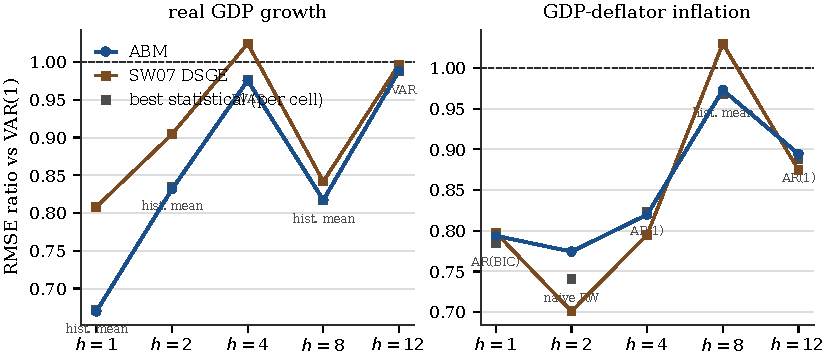
\includegraphics[width=\textwidth]{figures/f2_rmse_ratio_by_horizon.pdf}
\caption{\textbf{F2 --- RMSE ratio against horizon.} Left: real GDP growth --- the repair moves the
whole profile below the anchor and removes the $h=2$ spike. Right: GDP-deflator inflation --- the
two ABM curves are indistinguishable, because the reconciliation is a quantity intervention. Grey
squares mark the best statistical model \emph{in each cell separately}, with its identity
annotated; that envelope is a stiffer comparison than any single benchmark.
Data: \code{relative_scores.csv}, all-available track.}
\label{fig:f2}
\end{figure}

\begin{figure}[t]
\centering
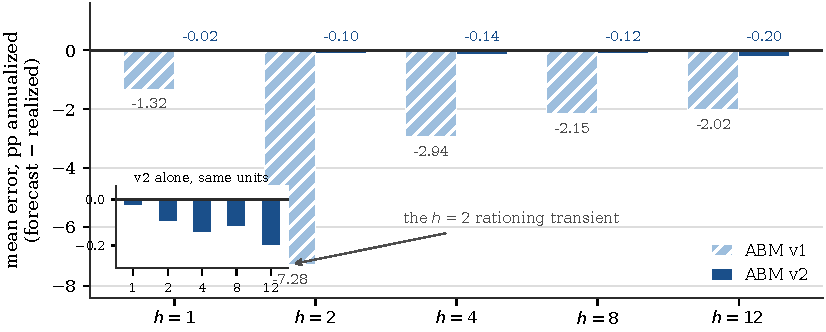
\includegraphics[width=\textwidth]{figures/f3_real_gdp_bias.pdf}
\caption{\textbf{F3 --- real-GDP mean error by horizon.} The first pass under-forecasts at every
horizon, with a $-7.28$\pp\ transient at $h=2$ that the diagnosis attributes to the rationing crash
rather than to the opening-row measurement basis. The repaired bars are barely visible at this
scale; the inset shows them on their own axis, where the largest residual bias is $-0.20$\pp.
Data: \code{score_summaries.csv}, all-available track.}
\label{fig:f3}
\end{figure}

\subsection{The mean-absolute-error asymmetry is resolved, not traded away}

The weighted MAE ratio moves from 1.137 to \textbf{0.814}. Per cell:

\begin{table}[h]
\centering
\caption{MAE ratios against the VAR(1) anchor, $h=1/2/4/8/12$. Every real- and nominal-GDP MAE
ratio is now below one at every horizon. The first pass's weak MAE column was neither a
functional-choice artifact nor an intrinsic property of ensemble forecasting: it was the 2\pp\
bias, which costs MAE proportionally more than it costs RMSE.}
\label{tab:mae}
\small
\begin{tabular}{@{}lll@{}}
\toprule
Target & v1 & \textbf{v2} \\
\midrule
\code{real_gdp} & 0.842 / \textbf{2.376} / 1.454 / 1.087 / 1.283 & \textbf{0.691 / 0.734 / 0.879 / 0.790 / 0.962} \\
\code{nominal_gdp} & 0.819 / \textbf{2.071} / 1.272 / 1.008 / 1.155 & \textbf{0.711 / 0.725 / 0.851 / 0.804 / 0.937} \\
\code{gdp_deflator} & 0.919 / 0.780 / 0.807 / 0.861 / 0.842 & 0.919 / 0.779 / 0.808 / 0.866 / 0.843 \\
EFFR & 0.584 / 0.627 / 0.664 / 0.762 / 0.777 & 0.584 / 0.627 / 0.663 / 0.762 / 0.775 \\
\bottomrule
\end{tabular}
\end{table}

\subsection{Density calibration}

A point forecast is only part of what a simulation ensemble produces. \emph{Interval coverage} asks
how often the realised value falls inside a stated predictive interval: a well-calibrated 90\,\%
interval should contain the truth 90\,\% of the time. Table~\ref{tab:coverage} and
Figure~\ref{fig:f4} report coverage pooled over all five horizons ($n=283$ per target).

\begin{table}[h]
\centering
\caption{Empirical interval coverage, pooled over five horizons, $n=283$ per target. Nominal
coverage is 0.90 / 0.80 / 0.50. Computed by $n$-weighted aggregation of the per-horizon rows in
\code{abm_v2_interval_coverage.csv}.}
\label{tab:coverage}
\footnotesize
\begin{tabular}{@{}lcccccc@{}}
\toprule
Target & v1 5--95\,\% & \textbf{v2 5--95\,\%} & v1 10--90\,\% & \textbf{v2 10--90\,\%} & v1 25--75\,\% & \textbf{v2 25--75\,\%} \\
\midrule
\code{real_gdp} & 0.654 & \textbf{0.929} & 0.580 & \textbf{0.894} & 0.300 & 0.696 \\
\code{nominal_gdp} & 0.661 & \textbf{0.890} & 0.548 & \textbf{0.830} & 0.332 & 0.608 \\
\code{gdp_deflator} & 0.742 & 0.735 & 0.703 & 0.703 & 0.449 & 0.470 \\
EFFR & 0.509 & 0.512 & 0.431 & 0.438 & 0.247 & 0.251 \\
\code{unemployment_rate} & 0.509 & \textbf{0.216} & 0.375 & \textbf{0.127} & 0.177 & 0.071 \\
\bottomrule
\end{tabular}
\end{table}

The repaired model's real-GDP density is well calibrated at the 90\,\% and 80\,\% levels (0.929 and
0.894 against nominal 0.90 and 0.80). The first pass's 0.654 and 0.580 were \emph{not} a width
problem --- the intervals missed because the point forecast was biased down by $\approx2$\pp.
Nominal GDP improves comparably. The 50\,\% band now over-covers (0.696 against 0.500): the centre
of the repaired ensemble is too wide.

Three targets remain badly calibrated and are named as open work. The deflator is under-dispersed
at every level and \emph{unchanged} by this work --- the ensemble's inflation spread is genuinely
too narrow. The policy rate under-covers badly and increasingly with horizon (0.754 at $h=1$ down to
0.200 at $h=12$) in both versions --- the Taylor-rule path is far too tight. Unemployment coverage
\emph{falls} and reaches exactly 0.000 at $h=12$, which is the defect of
\S\ref{sec:unemployment} appearing in the density as well as the mean. This is a coverage
assessment only: no probability-integral-transform histogram, log score or continuous ranked
probability score was computed, so it is not a full density evaluation.

\begin{figure}[t]
\centering
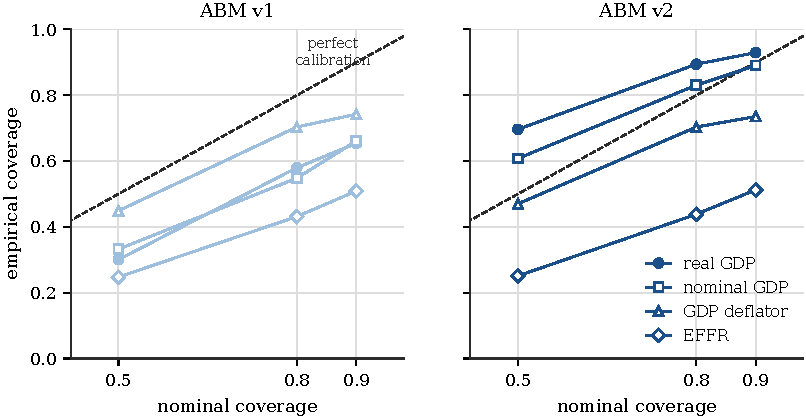
\includegraphics[width=\textwidth]{figures/f4_interval_coverage.pdf}
\caption{\textbf{F4 --- empirical against nominal interval coverage}, pooled over five horizons,
$n=283$ per target. Points on the dashed 45$^{\circ}$ line are perfectly calibrated; below the line
is over-confident. The repair lifts real and nominal GDP onto the line at the 80\,\% and 90\,\%
levels while leaving the deflator and the policy rate --- both under-dispersed --- where they were.
Data: \code{abm_v2_interval_coverage.csv}.}
\label{fig:f4}
\end{figure}

\begin{figure}[t]
\centering
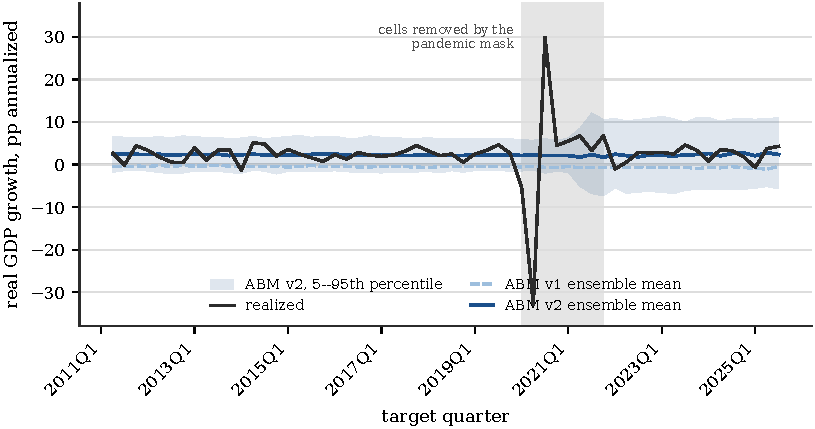
\includegraphics[width=\textwidth]{figures/f9_paths_h4.pdf}
\caption{\textbf{F9 --- four-quarter-ahead real GDP growth across the whole backtest.} Each point on
the model curves is the ensemble functional from a different origin. The first pass sits at
approximately zero growth throughout; the repaired model sits near $+2.3$\,\% and tracks the level
of realised growth. Neither forecasts the pandemic quarters, which is why the pandemic-masked track
exists. Only cells with a realised target quarter in the panel are shown, so the series ends at
2025Q3. Data: \code{abm_ensemble_summaries.csv} (both versions), \code{quarterly_panel.csv}.}
\label{fig:f9}
\end{figure}

\subsection{Secondary targets}

Nominal GDP growth is the exact sum of real GDP growth and deflator inflation, so it adds no
independent information but costs nothing to report. The policy-rate operator maps the model's
internal Taylor-rule rate to an annualised percentage point; \textbf{this is explicitly not an
approved EFFR bridge}, and the caveat travels with every number in Table~\ref{tab:secondary}.

\begin{table}[h]
\centering
\caption{Secondary target pair \{nominal GDP growth, effective federal funds rate\}, weighted RMSE
ratios. Weighted MAE ratios follow the same pattern: 0.717 / 0.694 / 0.735 for the repaired model
against 0.971 / 0.912 / 1.268 for the first pass.}
\label{tab:secondary}
\small
\begin{tabular}{@{}llllc@{}}
\toprule
Track & v2 mean (rank) & v2 median & v1 mean (rank) & Best statistical \\
\midrule
all-available & \textbf{0.716 (1st)} & 0.716 (2nd) & 0.782 (5th) & \code{univariate_ar_bic} 0.780 \\
balanced $h{=}12$ & \textbf{0.703 (1st)} & 0.704 (2nd) & 0.761 (4th) & \code{univariate_ar_bic} 0.770 \\
pandemic-masked & 0.739 (2nd) & 0.741 (3rd) & 1.124 (10th) & \textbf{\code{univariate_ar_p4} 0.719 (1st)} \\
\bottomrule
\end{tabular}
\end{table}

\textbf{The pandemic-masked loss is reported as a loss.} On the secondary pair in the calm sample,
AR(4) at 0.719 beats the repaired ABM at 0.739 --- a 2.8\,\% margin. The repaired model wins the
other two tracks and the headline pair everywhere, but it does not sweep the field, and the one
cell where a statistical model wins outright is stated here rather than buried.

\subsection{Unemployment: an open defect that became worse}
\label{sec:unemployment}

\code{unemployment_rate} is excluded from every weighted score in both versions, for the reason
recorded in each manifest: the initial unemployed stock is a length-one annual array frozen at 2024,
so every historical origin opens at the 2024 labour market.

\emph{The first-pass defect was a constant forecast.} Across all 61 origins the $h=1$ unemployment
forecast ranges from 3.492\,\% to 3.679\,\% --- a span of 0.187\pp, cross-origin standard deviation
0.048\pp\ --- against realised values spanning 3.533\,\% to 13.000\,\%. Had it been scored, the
first pass would have ranked 1st or 2nd of the 14 columns at $h=8$ and $h=12$. \emph{Those are not wins.} They
are a constant landing near the sample mean, and the giveaway is that
\code{naive_historical_mean} --- a constant by construction --- is the best statistical model in
exactly those cells.

\emph{The post-repair defect is collapse.} Once goods rationing stops, the labour block overheats.
Bias moves from $-1.97 / -0.86 / -0.06 / +0.19 / +0.08$\pp\ to
$-2.09 / -2.38 / -3.12 / -4.39 / -4.73$\pp, and MASE from $7.7 / 6.0 / 5.9 / 5.7 / 5.2$ to
$8.1 / 9.3 / 12.2 / 17.3 / 18.8$. End-of-horizon unemployment at four origins with 64 matched-seed
paths is 0.76--1.11\,\% under the reconciliation alone and 0.12--0.50\,\% with the expectation
change, against 4.73--5.28\,\% before. \textbf{This is not credible}, it is a direct consequence of
the repair, and it is the diagnosis's predicted side effect.

Two separable items of future work follow, and they should not be bundled. (a) Fetching historical
annual Current Population Survey series would remove the frozen-stock defect and make the target
scoreable at historical origins. (b) The post-reconciliation collapse is a labour-block behavioural
issue requiring its own diagnosis of the kind in \S\ref{sec:diagnosis}. \emph{(a) does not fix
(b).}

% ===========================================================================
\FloatBarrier
\section{The current outlook --- unscored}
\label{sec:outlook}

Two origins beyond the end of the revised panel --- 2025Q4 and 2026Q1 --- were run on the repaired
artifact with 500 paths and zero path failures. There is no realised truth for these, so
\textbf{nothing in this section is scored} (\code{scored = false},
\code{realized_truth_available = false}), and the headroom caveat of \S\ref{sec:headroom} applies
with more force at $h=12$ than inside the scored window.

From the 2025Q4 origin, average real growth over $h=1\ldots4$ is $+2.11\,\%$ with a 5th--95th
percentile band of roughly $-5.5$ to $+10$; deflator inflation runs $3.21\,\%$ at $h=1$, easing to
$2.40\,\%$ by $h=4$ and $\approx2.25\,\%$ by $h=12$; the policy rate declines from $3.86\,\%$ to
$3.32\,\%$. From the 2026Q1 origin, average real growth over $h=1\ldots4$ is $+2.31\,\%$, average
deflator inflation $+2.86\,\%$, and the policy rate declines from $3.60\,\%$ to $3.47\,\%$ by $h=4$
and $3.16\,\%$ by $h=12$. Figure~\ref{fig:f6} shows the 2026Q1 fan.

Two things to note when reading Figure~\ref{fig:f6}. First, the first-pass outlook's $-4.9\,\%$ dive
at $h=2$ is gone: it was the transient of \S\ref{sec:v1} and does not survive the balance fix.
Second, path dispersion is large \emph{by construction} --- the real-GDP ensemble standard deviation
is 4.6--5.1\pp, a 5th--95th band spanning $\approx16$\pp\ --- while the Monte-Carlo standard error of
the mean is $\approx0.2$\pp. The width is model dispersion, not simulation noise, and per
Table~\ref{tab:coverage} the real-GDP 90\,\% band is close to nominal coverage in backtest while
the deflator and policy-rate bands are demonstrably too narrow.

\begin{figure}[t]
\centering
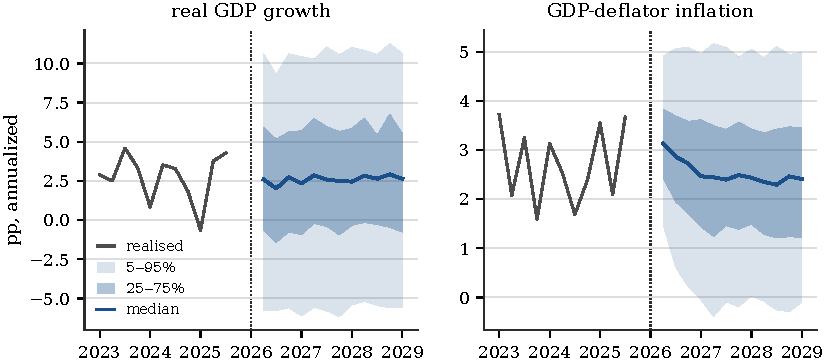
\includegraphics[width=\textwidth]{figures/f6_outlook_fan.pdf}
\caption{\textbf{F6 --- current outlook from the 2026Q1 origin, unscored.} Realised history from
2023Q1 is prepended in grey for context; the fan shows the ensemble median with 25--75th and
5--95th percentile bands over $h=1\ldots12$. The dotted line marks the origin. The deflator fan
narrows to a stable $\approx2.3\,\%$ median while the real-growth fan is essentially flat around
$+2\,\%$ with wide, roughly horizon-invariant dispersion --- the signature of a model whose
conditional uncertainty saturates quickly. Data: \code{current_outlook.csv},
\code{quarterly_panel.csv}.}
\label{fig:f6}
\end{figure}

% ===========================================================================
\FloatBarrier
\section{Limitations and open problems}
\label{sec:limits}

Ranked by inferential risk to the results above.

\subsection{Capacity-headroom growth ceiling --- no capital accumulation}
\label{sec:headroom}

\textbf{The most binding limitation on any forward use.} Investment is replacement-only and
$K_{\text{end}}/K_1 = 1.0000$ in every variant, so \emph{all} of the repaired model's extra growth
comes from draining the fixed 17.6\,\% opening capacity headroom implied by the hard-coded
$\omega=0.85$. Measured over 24 quarters at the 2016Q4 origin with 24 paths:

\begin{table}[h]
\centering
\caption{Six-year growth decomposition by variant, annualised by year. The rejected
``budgets-held'' closure exhausts its headroom in about four years and decays to $+0.33\,\%$/yr,
which is precisely why its smaller headline bias was not taken as evidence in its favour.}
\label{tab:headroom}
\small
\footnotesize
\begin{tabular}{@{}lrrrrrrcr@{}}
\toprule
Variant & y1 & y2 & y3 & y4 & y5 & y6 & Utilisation y1$\rightarrow$y6 & $K_{24}/K_0$ \\
\midrule
v1 baseline & $-1.62$ & $-0.04$ & 0.59 & 0.45 & 1.19 & 1.36 & $0.845\rightarrow0.865$ & 1.0003 \\
budgets held (rejected) & 3.33 & 3.60 & 3.53 & 2.71 & 1.39 & \textbf{0.33} & $0.867\rightarrow\mathbf{0.986}$ & 1.0000 \\
\textbf{v2 ($\lambda$ closure)} & 1.17 & 1.06 & 1.56 & 1.47 & 2.86 & 3.33 & $0.856\rightarrow\mathbf{0.943}$ & 1.0000 \\
\bottomrule
\end{tabular}
\end{table}

Inside the 12-quarter scoring window this is a genuine improvement. Beyond roughly eight to ten
years the repaired model must stall, because it has consumed 0.087 of its 0.144 headroom in six.
A capacity-expansion term in desired investment --- calibrated against the accounting identity
$\text{net } I = \Delta K$, \emph{never} against forecast RMSE --- is the prerequisite for any
multi-year use. \textbf{The repaired model is validated at $h \le 12$ only, and is not a multi-year
growth mechanism.}

\subsection{The labour block}
Two distinct failures, as set out in \S\ref{sec:unemployment}: a frozen 2024 opening stock, and a
post-repair collapse to $\approx1\,\%$ unemployment. Fixing the first does not fix the second, and
the labour block needs its own diagnosis before unemployment is scored for either version.

\subsection{Mixed-vintage structure and a single structural year}
The 2024 input--output structure, firm and employee counts, tax rates and population are future
information at every origin before 2024. This is bounded for flow targets and fatal for
stock-initialised ones, and it is the limitation that most sharply separates this exercise from the
reference paper. Separately, even setting look-ahead aside, the model has \emph{one} technology
matrix for a fifteen-year sample: real changes in U.S.\ production structure over 2010--2025 --- the
energy mix, the information-sector share, post-2020 supply-chain reconfiguration --- are invisible
to it by construction. This limits what the sector-level diagnostics of \S\ref{sec:diagnosis} can be
asked to bear, and it is a reason to treat the reconciled 2024 table as a \emph{fixed technology}
rather than a historical one.

\subsection{Absent bridges: PCE, core PCE, payroll employment}
Three of the eight registered targets are unserved. The personal consumption expenditures price
index and its core variant need a consumption-basket price bridge that the 68-commodity model does
not expose, and the core additionally needs a food/energy exclusion the classification does not
identify cleanly. Payroll employment targets an establishment count on a different universe from the
model's firm employment. None should be scored until a bridge qualification of the kind done for the
GDP operator is complete. The practical cost is that the model is compared on five of eight targets,
and the semi-structural comparator's core-four target set cannot be matched.

\subsection{Density evaluation is partial; the scale ladder was not run for the headline}
\S\ref{sec:v2} reports interval coverage only. Moreover all headline results are at scale
$10^{-5}$ (130 firms). The scale sweep established that the \emph{mean} bias is invariant from 130
to 2\,708 firms, but 54 of 68 sectors hold exactly one firm at this scale, which makes
cross-sectional dispersion and tail behaviour unreliable. A production run at scale $\ge10^{-4}$
costs roughly $8\times$ the runtime and should precede any density claim.

\subsection{No DSGE benchmark; the semi-structural comparator is not in the field}
The reference paper compares its ABM against a Bayesian DSGE model of the
\citet{smetswouters2007} family; this exercise does not. A small New-Keynesian design exists in the
repository and the Federal Reserve Bank of New York's open-source DSGE model is the natural external
candidate. Until one is scored on this grid, ``best in the field'' means \emph{best among ten
time-series benchmarks}. Adding the semi-structural Kalman comparator under the ABM's target set is
the cheaper first step.

\subsection{Inference}
No formal inference was performed: no \citet{dieboldmariano1995} test, no
heteroskedasticity-and-autocorrelation-consistent adjustment, no bootstrap, and no
multiple-comparison control across the $14 \times 5 \times 5 \times 3$ grid of models, targets,
horizons and tracks. The rankings are descriptive. The version contrast is the most defensible
comparison in this paper because it is matched-seed on identical cells with one deliberate change;
the comparisons against statistical models are not, and margins of a few per cent --- such as 0.830
against \code{naive_historical_mean}'s 0.879 --- should not be treated as established.

\subsection{Residual reproducibility notes}
The pipeline's baseline builder errors out and cannot regenerate its own baselines; the checked-in
artifacts load and run correctly, so this does not block the work, but the provenance chain is
broken at the regeneration step. The reconciliation builder is deliberately standalone and is not
wired into the artifact-build entry point for that reason. Minor: the Monte-Carlo error file in the
repaired run's output directory carries a stale first-pass model-family label on rows that are the
repaired ensemble's own errors; the values are correct, only the family string is wrong, and no
reported number depends on it. Finally, the narrative in the repository's results report states 543
RAS iterations where the committed reconciliation report states 623; the committed artifact is
authoritative and Table~\ref{tab:ras} follows it.

\subsection{Pointer to a vintage-clean design}
A stage-3, pseudo-real-time design requires year-by-year annual history for the 37 frozen arrays
--- BEA input--output summary use/make tables after redefinitions; Census SUSB and BLS QCEW for
firms and employees per sector; BLS CPS for population, unemployed and inactive; BEA national
income and product accounts for tax and benefit aggregates, and BEA fixed-assets tables for assets,
dwellings and capital consumption \citep{bea_nipa} --- plus a real-time truth layer of the \citet{croushorestark2001} kind, for which a
Philadelphia Fed real-time data set capture already exists on disk. Quarterly series need no fetch;
they run from 1996Q4. This is a data-acquisition programme, not a modelling one, and it is the only
route to a promotion claim. A realistic first cut restricts origins to 2014 and later, where the
annual coverage is densest.

% ===========================================================================
\FloatBarrier
\section{Conclusion}
\label{sec:conclusion}

An agent-based macroeconomic model of the United States was calibrated from public source data,
scored against ten statistical benchmarks on a matched grid of 61 quarterly origins and five
horizons with 500 free-running paths per origin, found to carry a large and systematic real-growth
bias, diagnosed by matched-seed experiment to two specific defects, repaired by restoring an
accounting identity and correcting a misspecified estimator --- neither repair \emph{selected}
using forecast errors --- and then re-scored on identical cells with identical seeds. The exercise
remains explicitly mixed-vintage: 2024 structure and current-vintage data are used at historical
origins. That arc
is the result. The rank improvement is a consequence of it, not the object of it.

Three findings are worth carrying away.

\emph{First, the defect was in the accounting, not the behaviour.} A supply--use system that
balances in its published valuation basis need not balance after a valuation bridge and an
industry-to-commodity projection, and an agent-based model with a fixed capacity envelope and a
one-sided production constraint has no mechanism that can absorb the difference. The failure mode
was not a badly chosen parameter; it was an identity that had quietly stopped holding. This is a
class of failure that structural simulators are especially exposed to and that a reduced-form model,
having no accounting identities to violate, cannot exhibit.

\emph{Second, the diagnosis made a falsifiable out-of-sample prediction, and it held.} The
mechanism implied a real quantity-rationing defect and therefore predicted that the price block
would be untouched by the repair. The GDP deflator's $h=1$ cell is bit-identical between the two
versions, and its ratios differ in the third decimal at every other horizon, while real-GDP bias
falls by two orders of magnitude. A diagnosis that predicts what will \emph{not} change is more
informative than one that only predicts what will.

\emph{Third, the improvement is bounded by a defect that was not repaired.} All of the repaired
model's growth drains a fixed 17.6\,\% capacity headroom, because investment is replacement-only and
capital never accumulates. Within the twelve-quarter scoring window this is a genuine improvement;
beyond roughly eight to ten years it is not a growth mechanism at all. Reporting the rank without
this caveat would misrepresent what has been established.

What has been established is that a specific, located, repairable accounting defect explained a
2-percentage-point forecast bias, and that after repair the model attains the lowest weighted RMSE
ratio in a fourteen-column field on the headline target pair in all three sample tracks. What has
not been established is real-time forecast skill, validity beyond twelve quarters, anything about
the labour block, or statistical separation from the models ranked immediately below. The route
from here is a data-acquisition programme for vintage-correct structural inputs, a capacity
expansion term calibrated against the investment identity, and a labour-block diagnosis of the kind
performed here for the goods market.

% ===========================================================================
\appendix
\section{Reproducibility}
\label{app:repro}

\subsection{Commands}

All commands run from the repository root. Both environment variables are hard requirements on the
benchmark path: the runner raises an error unless the Julia and BLAS thread counts are both 1.

\begin{quote}\small\ttfamily
\# 1. build the reconciled calibration artifact ($\sim$40\,s)\\
julia --project=scripts/us \textbackslash\\
\hspace*{2em}scripts/us/calibration/reconcile\_commodity\_balance.jl \textbackslash\\
\hspace*{2em}--mode=final\_demand\_scaled --expectations=rw\_drift\\[4pt]
\# 2. the two ensembles, 61 origins $\times$ 500 paths each\\
JULIA\_NUM\_THREADS=1 OPENBLAS\_NUM\_THREADS=1 julia --project=scripts/us \textbackslash\\
\hspace*{2em}scripts/us/forecasting/diagnostics/abm\_revised\_comparison/\textbackslash\\
\hspace*{2em}run\_revised\_data\_abm\_comparison.jl \textbackslash\\
\hspace*{2em}output/us\_forecasting/abm\_v2\_comparison/v1\_headline 500 headline\\
\hspace*{2em}\ldots{} v2\_headline 500 headline\_v2\\[4pt]
\# 3. joint scoring: both ABM columns on identical common cells\\
\hspace*{2em}\ldots{} v2\_headline 500 headline\_v2 --also-score=\ldots/v1\_headline\\[4pt]
\# 4. current outlook (unscored)\\
\hspace*{2em}\ldots{} output/us\_forecasting/abm\_v2\_comparison\_outlook 500 outlook\_v2\\[4pt]
\# 5. figures for this paper\\
python3 paper/figures\_src/make\_figures.py\\[4pt]
\# 6. this paper\\
cd paper \&\& latexmk -pdf US\_ABM\_Forecasting\_Paper.tex
\end{quote}

Step~2 resumes from its own ensemble cache, so an interrupted run continues rather than restarting;
step~3 is a re-score off the cache (about 15\,s) rather than a re-simulation. Every figure in this
paper is regenerated by step~5 directly from the committed CSVs listed in
\S\ref{app:artifacts}; no figure contains a hand-entered number, and the generator pins
\code{SOURCE_DATE_EPOCH} so that a re-run reproduces each figure byte for byte.

\subsection{Artifact paths}
\label{app:artifacts}

\begin{table}[h]
\centering
\small
\footnotesize
\begin{tabular}{@{}>{\raggedright\arraybackslash}p{0.38\textwidth}>{\raggedright\arraybackslash}p{0.56\textwidth}@{}}
\toprule
Path (under the repository root) & Contents \\
\midrule
\pathc{output/us_forecasting/abm_v2_comparison/v2_headline/}
& the canonical scored result: both ABM columns, 14 forecast columns, 500 paths ---
  \code{manifest.toml}, \code{score_summaries.csv}, \code{relative_scores.csv},
  \code{weighted_relative_scores.csv}, \code{monte_carlo_errors.csv},
  \code{abm_v2_interval_coverage.csv}, \code{abm_ensemble_summaries.csv},
  \code{abm_origin_diagnostics.csv}, \code{failures.csv} \\
\pathc{output/us_forecasting/abm_v2_comparison/v1_headline/}
& first-pass ensemble cache, re-run under the patched tree (gate G4) \\
\pathc{output/us_forecasting/abm_v2_comparison_outlook/}
& 2025Q4 and 2026Q1 origins on the reconciled artifact, unscored \\
\pathc{output/us_forecasting/commodity_balance_reconciliation/}
& \code{reconciliation_report_rho1.txt}, \code{reconciliation_by_commodity_rho1.csv} \\
\pathc{scripts/us/forecasting/diagnostics/revised_data/fixtures/quarterly_panel.csv}
& the scoring panel: 101 quarters, 2000Q3--2025Q3 \\
\pathc{paper/figures_src/make_figures.py}
& the figure generator for this paper \\
\bottomrule
\end{tabular}
\end{table}

\subsection{Commit hashes and identity seals}

\begin{table}[h]
\centering
\small
\begin{tabular}{@{}ll@{}}
\toprule
Commit & Content \\
\midrule
\code{a55d9ed} & checkpoint before the ABM campaign; the base all gates compare against \\
\code{9430a4a} & first-pass comparison: ABM against statistical benchmarks \\
\code{cd22674} & random-walk-drift expectations patch (flag-gated, default off) \\
\code{b82680e} & RAS reconciliation of the opening commodity balance $+$ reconciled artifact \\
\code{aadde2b} & repaired-model comparison run \\
\code{107a9ef} & merge of the repaired line \\
\code{461cdc3} & results report, from which this paper's narrative is drawn \\
\bottomrule
\end{tabular}
\end{table}

Table~\ref{tab:seals} lists the fields sealed in every repaired-run manifest. For contrast,
the first-pass calibration object is \pathc{data/us/calibration/US_2024_calibration_object.jld2}
with SHA-256 \code{4cce5d62...05e2e136}.

\begin{table}[h]
\centering
\footnotesize
\begin{tabular}{@{}>{\raggedright\arraybackslash}p{0.36\textwidth}>{\raggedright\arraybackslash}p{0.58\textwidth}@{}}
\toprule
Manifest field & Value \\
\midrule
\code{calibration_object_path} & \pathc{data/us/calibration/US_2024_calibration_object_reconciled.jld2} \\
\code{calibration_object_sha256} & \code{57e23f4a...e514760} \\
\code{commodity_balance_reconciled} & \code{true} \\
\code{reconciliation_mode} & \code{final_demand_scaled} \\
\code{reconciliation_rho} & \code{1.0} \\
\code{reconciliation_lambda} & \code{0.9834601934561227} \\
\code{growth_expectation_specification} & \code{rw_drift} \\
\code{monte_carlo_paths} / \code{burn_in_quarters} / \code{simulated_quarters} & \code{500} / \code{0} / \code{12} \\
\code{model_count} & \code{14} \\
\code{panel_sha256} & \code{f7bb26a4...bff851bbe} \\
\code{julia_version} / \code{julia_threads} / \code{blas_threads} & \code{1.10.3} / \code{1} / \code{1} \\
\bottomrule
\end{tabular}
\caption{Identity seals recorded by the runner in the repaired run's manifest.}
\label{tab:seals}
\end{table}

The $\lambda$ semantics recorded verbatim in each manifest read: \emph{``explicit accounting choice:
the four final-demand aggregates C, G, I and X (and capital\_\allowbreak consumption and
gross\_\allowbreak capitalformation\_\allowbreak dwellings, which set the investment budget) are
scaled by lambda so the
artifact's expenditure aggregates match its production account and the opening commodity balance
clears exactly. lambda is fixed by the accounting identity alone and was not chosen with reference
to any forecast error.''}

\subsection{Seed policy}

\begin{itemize}[leftmargin=1.4em,itemsep=1pt]
\item Simulation seeds are $\mathrm{hash}((\texttt{:abm\_revised\_v1},\,\text{origin},\,
      \text{path}))\bmod 2^{30}$: domain-separated by origin and path, so no two cells share a
      stream.
\item The repaired model draws the \emph{identical} seed stream as the first pass, which makes the
      contrast matched-seed. The expectations patch consumes exactly one Normal variate on either
      branch to preserve this.
\item The seed is set \emph{immediately before} model construction, because the initial microstate
      is drawn from the global generator; seeding after construction yields a random initial state
      and is a silent error. A fresh model is constructed per path; the library's built-in
      ensemble runner is not used, because it deep-copies one already-constructed model and would
      give every path the same initial microstate.
\item Diagnosis experiments use a separate domain-separated seed family, identical across every
      variant.
\item Failed paths are counted and left visible, never resampled. The count is 0 in every run.
\end{itemize}

\bibliography{refs}

\end{document}
